% Options for packages loaded elsewhere
\PassOptionsToPackage{unicode}{hyperref}
\PassOptionsToPackage{hyphens}{url}
%
\documentclass[
  a4paper,
]{scrbook}

\usepackage{amsmath,amssymb}
\usepackage{setspace}
\usepackage{iftex}
\ifPDFTeX
  \usepackage[T1]{fontenc}
  \usepackage[utf8]{inputenc}
  \usepackage{textcomp} % provide euro and other symbols
\else % if luatex or xetex
  \usepackage{unicode-math}
  \defaultfontfeatures{Scale=MatchLowercase}
  \defaultfontfeatures[\rmfamily]{Ligatures=TeX,Scale=1}
\fi
\usepackage{lmodern}
\ifPDFTeX\else  
    % xetex/luatex font selection
  \setmainfont[]{Latin Modern Roman}
  \setsansfont[]{Latin Modern Roman}
\fi
% Use upquote if available, for straight quotes in verbatim environments
\IfFileExists{upquote.sty}{\usepackage{upquote}}{}
\IfFileExists{microtype.sty}{% use microtype if available
  \usepackage[]{microtype}
  \UseMicrotypeSet[protrusion]{basicmath} % disable protrusion for tt fonts
}{}
\makeatletter
\@ifundefined{KOMAClassName}{% if non-KOMA class
  \IfFileExists{parskip.sty}{%
    \usepackage{parskip}
  }{% else
    \setlength{\parindent}{0pt}
    \setlength{\parskip}{6pt plus 2pt minus 1pt}}
}{% if KOMA class
  \KOMAoptions{parskip=half}}
\makeatother
\usepackage{xcolor}
\setlength{\emergencystretch}{3em} % prevent overfull lines
\setcounter{secnumdepth}{5}
% Make \paragraph and \subparagraph free-standing
\ifx\paragraph\undefined\else
  \let\oldparagraph\paragraph
  \renewcommand{\paragraph}[1]{\oldparagraph{#1}\mbox{}}
\fi
\ifx\subparagraph\undefined\else
  \let\oldsubparagraph\subparagraph
  \renewcommand{\subparagraph}[1]{\oldsubparagraph{#1}\mbox{}}
\fi


\providecommand{\tightlist}{%
  \setlength{\itemsep}{0pt}\setlength{\parskip}{0pt}}\usepackage{longtable,booktabs,array}
\usepackage{calc} % for calculating minipage widths
% Correct order of tables after \paragraph or \subparagraph
\usepackage{etoolbox}
\makeatletter
\patchcmd\longtable{\par}{\if@noskipsec\mbox{}\fi\par}{}{}
\makeatother
% Allow footnotes in longtable head/foot
\IfFileExists{footnotehyper.sty}{\usepackage{footnotehyper}}{\usepackage{footnote}}
\makesavenoteenv{longtable}
\usepackage{graphicx}
\makeatletter
\def\maxwidth{\ifdim\Gin@nat@width>\linewidth\linewidth\else\Gin@nat@width\fi}
\def\maxheight{\ifdim\Gin@nat@height>\textheight\textheight\else\Gin@nat@height\fi}
\makeatother
% Scale images if necessary, so that they will not overflow the page
% margins by default, and it is still possible to overwrite the defaults
% using explicit options in \includegraphics[width, height, ...]{}
\setkeys{Gin}{width=\maxwidth,height=\maxheight,keepaspectratio}
% Set default figure placement to htbp
\makeatletter
\def\fps@figure{htbp}
\makeatother

\usepackage{booktabs}
\usepackage{longtable}
\usepackage{array}
\usepackage{multirow}
\usepackage{wrapfig}
\usepackage{float}
\usepackage{colortbl}
\usepackage{pdflscape}
\usepackage{tabu}
\usepackage{threeparttable}
\usepackage{threeparttablex}
\usepackage[normalem]{ulem}
\usepackage{makecell}
\usepackage{xcolor}
\usepackage{fancyhdr}
\usepackage{textcomp}
\usepackage{titling}
\usepackage{pdflscape}
\usepackage{rotating}
\usepackage{geometry}
\usepackage{setspace}
\setlength{\droptitle}{-2cm}
\preauthor{
  \begin{center}
  \Large
  \vspace{15mm}
  by
  \vspace{10mm}
  
}
\postauthor{
  \end{center}
  
}

\predate{
  \begin{spacing}{1.2}
  \begin{center}
  \vspace{22mm}
  
  A thesis \\
  submitted to the Victoria University of Wellington \\
  in partial fulfilment of the requirements for the  \\
  degree of Doctor of Philosophy\\               % Degree
  \vspace{24mm}
  Te Herenga Waka $-$ Victoria University of Wellington\\
}
\postdate{
  \\
  
\includegraphics[width=3in,height=1.5in]{figures/VUW-logo.png}\\
  \end{center}
  \end{spacing}
  }

\renewcommand{\topfraction}{.8}
\renewcommand{\bottomfraction}{.7}
\renewcommand{\textfraction}{.15}
\renewcommand{\floatpagefraction}{.8}
\setcounter{topnumber}{3}
\setcounter{bottomnumber}{3}
\setcounter{totalnumber}{4}

\clubpenalty=9996
\widowpenalty=9999
\makeatletter
\makeatother
\makeatletter
\@ifpackageloaded{bookmark}{}{\usepackage{bookmark}}
\makeatother
\makeatletter
\@ifpackageloaded{caption}{}{\usepackage{caption}}
\AtBeginDocument{%
\ifdefined\contentsname
  \renewcommand*\contentsname{Table of contents}
\else
  \newcommand\contentsname{Table of contents}
\fi
\ifdefined\listfigurename
  \renewcommand*\listfigurename{List of Figures}
\else
  \newcommand\listfigurename{List of Figures}
\fi
\ifdefined\listtablename
  \renewcommand*\listtablename{List of Tables}
\else
  \newcommand\listtablename{List of Tables}
\fi
\ifdefined\figurename
  \renewcommand*\figurename{Figure}
\else
  \newcommand\figurename{Figure}
\fi
\ifdefined\tablename
  \renewcommand*\tablename{Table}
\else
  \newcommand\tablename{Table}
\fi
}
\@ifpackageloaded{float}{}{\usepackage{float}}
\floatstyle{ruled}
\@ifundefined{c@chapter}{\newfloat{codelisting}{h}{lop}}{\newfloat{codelisting}{h}{lop}[chapter]}
\floatname{codelisting}{Listing}
\newcommand*\listoflistings{\listof{codelisting}{List of Listings}}
\makeatother
\makeatletter
\@ifpackageloaded{caption}{}{\usepackage{caption}}
\@ifpackageloaded{subcaption}{}{\usepackage{subcaption}}
\makeatother
\makeatletter
\@ifpackageloaded{tcolorbox}{}{\usepackage[skins,breakable]{tcolorbox}}
\makeatother
\makeatletter
\@ifundefined{shadecolor}{\definecolor{shadecolor}{rgb}{.97, .97, .97}}
\makeatother
\makeatletter
\makeatother
\makeatletter
\makeatother
\ifLuaTeX
  \usepackage{selnolig}  % disable illegal ligatures
\fi
\usepackage[citestyle = ieee,urldate = iso8601]{biblatex}
\addbibresource{references.bib}
\IfFileExists{bookmark.sty}{\usepackage{bookmark}}{\usepackage{hyperref}}
\IfFileExists{xurl.sty}{\usepackage{xurl}}{} % add URL line breaks if available
\urlstyle{same} % disable monospaced font for URLs
\hypersetup{
  pdftitle={Developing an Insect Odorant Receptor Bioelectronic Nose for Vapour-Phase Detection},
  pdfauthor={Eddyn Oswald Perkins Treacher},
  hidelinks,
  pdfcreator={LaTeX via pandoc}}

\title{Developing an Insect Odorant Receptor Bioelectronic Nose for
Vapour-Phase Detection}
\author{Eddyn Oswald Perkins Treacher}
\date{Dec 2024}

\begin{document}
\frontmatter

\maketitle

\begin{spacing}{1.2}

\clearpage
\newpage
\thispagestyle{empty} % Hide header and footer on this page
\mbox{~}
\clearpage
\newpage

%----------------------------------------------
%   Abstract
%----------------------------------------------

\thispagestyle{plain}

\begin{flushleft}
% Manually add a section to the table of contents
\pagenumbering{roman}
\addcontentsline{toc}{chapter}{Abstract}
\huge\textbf{Abstract}
\end{flushleft}

\vspace*{\baselineskip}

The ability to detect volatile organic compounds in a highly sensitive and selective manner could be used for applications as varied as diagnoses of illnesses at a remote clinic, monitoring of air in an industrial setting, or identification of invasive organisms at a biosecurity checkpoint. Historically, animal noses have been used for such tasks, as their combined sensitivity and selectivity are superior to traditional artificial sensors. However, training and deploying animals in such situations is both time and cost intensive. In recent years, an improved understanding of \textit{in vivo} biological sensing has driven efforts to mimic these highly efficient processes in an artificial sensor format. \\[5pt] To this end, a ``bioelectronic nose'' was developed. This sensor uses an artificial transducer to amplify responses of an insect odorant receptor protein to specific volatile compounds. Thin-film transistors were used as the amplifier element, given their low cost, small size and extreme sensitivity. Various thin-film morphologies were compared, and their suitability for bioelectronic nose development assessed. Transducers made using a novel steam-assisted thin-film deposition technique were found to have highly consistent device-to-device electrical properties relative to other films. Films made using this process typically showed more surface contamination than other morphologies, but their high sensitivity was confirmed with a non-specific sensing series in an aqueous environment. \\[5pt] One of the major challenges encountered in this thesis was variability in the quality of sensor functionalisation. Raman spectroscopy and fluorescence microscopy were used to confirm an existing non-covalent attachment method could successfully immobilise nanodiscs onto the transistor channel region. However, various sensors functionalised using the same procedure often exhibited no sensing activity. Extensive electrical characterisation indicated the presence of an unidentified contamination layer which prevented electrical interaction between the insect odorant receptors and the transducer thin-film. It was shown that this layer was unlikely to be directly associated with the thin-film morphology used for the transducer. \\[5pt] Subsequently, an alternative biotin-based non-covalent method was used for functionalisation of the proteins, which eliminated several possible sources of contamination. This alternative biotin-based method was used to demonstrate successful aqueous sensing \newpage
\fancyhf{} %clear all headers and footers fields
\thispagestyle{fancy} % Change header and footer on this page
\renewcommand{\headrulewidth}{0pt}
\fancyhead[L]{\textit{Abstract}} % Set header content
\fancyfoot[L]{\thepage} %prints the page number on the left side of the header
of femtomolar concentrations of methyl salicylate by an iOR10a-functionalised device. When tested in a custom-built vapour delivery system, a similar bioelectronic sensor was shown to be highly sensitive to the target vapour. However, consistent reproduction of the biotin-based method was challenging due to the harsh cleaning method involved. It was therefore difficult to determine conclusively whether the vapour-phase sensor responses were selective. By finding new, systematic approaches to address the barriers to sensor success carefully identified in this work, there are promising signs that a highly reliable vapour-phase bioelectronic nose can be produced.

\clearpage
\newpage

%----------------------------------------------
%   Acknowledgement
%----------------------------------------------

\thispagestyle{plain}

\begin{flushleft}
% Manually add a section to the table of contents
\addcontentsline{toc}{chapter}{Acknowledgements}
\huge\textbf{Acknowledgements}
\end{flushleft}

\vspace*{\baselineskip}

I would first like to acknowledge the lands of my ancestors, and the lands of the sovereign first peoples to which my ancestors travelled. We each come from the land, live off the land and return to the land.
\end{spacing}
\begin{spacing}{1.2} 
\textit{Noon of Essex to Warrang, on the Friends, Autumn 1811} \\[5pt]
\textit{Cave of Cambridgeshire to Warrang, on the Royal Charlotte, Autumn 1825} \\[5pt]
\textit{Boyce of Suffolk to Warrang, 1832} \\[5pt] 
\textit{Charlton of Northumberland to Warrang, on the Clyde, Spring 1834} \\[5pt]
\textit{Prouse of Devonshire to Pito-one, on the Duke of Roxburgh, Summer 1840} \\[5pt]
\textit{Ebden of Devonshire to Pito-one, on the Tyne, Winter 1841} \\[5pt]
\textit{Collis of Hampshire to Pito-one, on the Birman, Autumn 1842} \\[5pt]
\textit{Swann of Loch Garman to Te Whanganui-a-Tara, 1844} \\[5pt] 
\textit{Blythe of Berkshire to Whakatū, circa 1846} \\[5pt]
\textit{Innes of Berkshire to Naarm, on the Sacramento, Autumn 1853} \\[5pt]
\textit{Sheppard of Gloucestershire to Naarm, 1853} \\[5pt] 
\textit{Bruce of London to Naarm, on the Omega, Autumn 1855} \\[5pt]
\textit{Quennell of Surrey to Warrang, on the Asiatic, Winter 1855} \\[5pt]
\textit{Barr of Glasgow to Kōpūtai, on the Sir Edward Paget, Winter 1856} \\[5pt] 
\textit{Perkins of London to Te Whanganui-a-Tara, on the Matoaka, Spring 1859} \\[5pt]
\textit{McKee of Antrim to Tāmaki Makaurau, on the Indian Empire, Spring 1862} \\[5pt]
\textit{Sandilands of Peeblesshire to Ōtepoti, circa 1864} \\[5pt] 
\textit{Treacher of Berkshire to Te Whanganui-a-Tara, on the Wild Duck, Summer 1865} \\[5pt]
\textit{McTaggart of Argyllshire to Kōpūtai, on the Edward P. Bouverie, Autumn 1869} \\[5pt] 
\textit{Chapman of Kent to Whakatū, on the Adamant, Winter 1874} \\[5pt]
\textit{Cheel of London to Whakatū, on the Queen Bee, Winter 1877} \\[5pt]  
\textit{Hutchison of Aberdeen to Tarntanya, before 1882.}
\end{spacing}
\begin{spacing}{1.2} 
\newpage
\fancyhf{} %clear all headers and footers fields
\thispagestyle{fancy} % Change header and footer on this page
\renewcommand{\headrulewidth}{0pt}
\fancyhead[L]{\textit{Acknowledgements}} % Set header content
\fancyfoot[L]{\thepage} %prints the page number on the left side of the header 
I chose to start my doctoral studies just a few months into a global pandemic. Completing a challenging project with a worldwide crisis in the background might have been impossible without the supervision of AProf. Natalie Plank. Her ability to adapt to and overcome any problem has taught me that there is no situation which is truly unmanageable. I am deeply grateful for her leadership throughout a time of particular chaos. \\[5pt] I started this project with minimal formal training in biological science, coming from a primarily physics and engineering background. The immense support I received from Melissa Jordan and Colm Carraher from the Institute for Plant and Food Research (PFR) to complete this project meant that this was not an issue, and I thank them both for this. \\[5pt] I would not have been able to begin this thesis without the financial backing and support I received from PFR and the Better Border Biosecurity (B3) programme. In particular, I am very grateful to Andrew Kralicek, formerly with PFR and now at Scentian Bio, and the ex-Director of B3, David Teulon, for helping to secure funding for my project. I would also like to thank the donor of the Ernest Marsden Scholarship in Physics for their significant financial support. \\[5pt] There are many incredibly supportive people who I worked alongside during my project. I would like to start off by thanking Rifat Ullah, whose mentoring and kindness encouraged me to pursue further study. His work on the initial design and setup of the vapour delivery system was invaluable to me throughout this project. I am also especially grateful to Alex Puglisi, for constructing the mechanical elements of the vapour delivery system and giving me extensive feedback on the system design. I would like to thank Peter Coard, for his advice and guidance when constructing the electrical elements of the vapour delivery system. I thank Selvan Murugathas, too, for his advice on constructing the insect odorant receptor sensors, as well as Damon Colbert and Valentina Lucarelli, who provided the insect odorant receptor nanodiscs used in this work. \\[5pt] Thank you to Prof. Ben Ruck, my supportive secondary supervisor, and to AProf. Franck Natali, for always asking about my thesis in the tearoom. Thank you to Gideon Gouws for his friendly encouragement and advice. For their substantial technical assistance and mentoring during this project, I thank Alan Rennie, Grant Franklin, Chris Lepper, Rashika Gunasekara, Pete Jebson and Sushila Pillai from VUW, Andrew Chan from PFR, AProf. Charles Unsworth from the University of Auckland, and Prof. Simon Brown and his nanomaterials group from the University of Canterbury. \\[5pt] I was lucky enough to start my doctoral program just as a group of supportive and talented senior students were finishing, and finished just as a group of enthusiastic and talented new doctoral students were starting. A special thanks to Jenna Nyugen, Erica Happe and Erica Cassie for teaching me the fabrication processes and characterisation procedures that made this thesis happen; and a special thanks to Marissa Dierkes, Danica Fontein, Sangar Begzaad and Alireza Zare, for their incredible support throughout the thesis writing process. I am also thankful for the assistance of the cleanroom group interns over the course of my PhD, including Liam, Hayden and Lotte. I would further like to thank everyone else I shared an office with and worked alongside, including Jackson, Will, Roshni, Ali, Sam, Kira, Catherine, Martin, Janani, Ted, Kiri and Joe. \\[5pt] A massive thank you to Openstar Technologies. It has been an honour to work on a cutting-edge plasma physics project right here in Te Whanganui-a-Tara. A particularly big thank you to Ratu, Darren and Thomas for having me as part of the plasma physics team. Thank you also to the other Openstar interns, in particular the other plasma physics interns, Valentina, Benjy and Chris. I wish you success in all your dipole-confined plasma related endeavours. \\[5pt] I want to thank Shodokan Aikido New Zealand for their support throughout this thesis, in particular for the once-in-a-lifetime opportunity to travel to Osaka to be graded for first-dan by Nariyama Shihan. Thanks for all the training and support, Ian. \\[5pt] Thank you to all the friends and whānau, old and new, who have supported me over these wild past few years. You know who you are. \\[5pt] Thank you to my brother, Keeson, and to my parents, Hilary and Phillip. Your support means everything to me, and I would not be where I am today without you. Our Friday lunchtime cafe visits kept me motivated and inspired throughout the doctoral program. Thank you, thank you, thank you for your love, your compassion, and for being there for me. \\[5pt] Finally, thank you Nina. Your incredible love has kept me going through the most difficult and most wonderful times over the last four years. You are the light of my life, and I am so happy to have taken on this challenge with you by my side. \\[5pt] Arohanui and peace to you all, Eddyn (Ned)

\fancyhf{} %clear all headers and footers fields
\thispagestyle{fancy} % Change header and footer on this page
\renewcommand{\headrulewidth}{0pt}
\fancyhead[R]{\textit{Acknowledgements}} % Set header content
\fancyfoot[R]{\thepage} %prints the page number on the right side of the header

\clearpage
\newpage
\thispagestyle{empty} % Hide header and footer on this page
\mbox{~}
\clearpage
\newpage

\pagestyle{headings}

\end{spacing}\ifdefined\Shaded\renewenvironment{Shaded}{\begin{tcolorbox}[frame hidden, boxrule=0pt, interior hidden, sharp corners, borderline west={3pt}{0pt}{shadecolor}, enhanced, breakable]}{\end{tcolorbox}}\fi

\begin{spacing}{1.2}

\renewcommand*\contentsname{Table of Contents}
{
\setcounter{tocdepth}{2}
\addcontentsline{toc}{chapter}{Table of Contents}
\tableofcontents
}
\listoffigures
\addcontentsline{toc}{chapter}{List of Figures}
\listoftables
\addcontentsline{toc}{chapter}{List of Tables}

\clearpage
\newpage

%----------------------------------------------
%   List of Abbreviations
%----------------------------------------------

\thispagestyle{plain}

\begin{flushleft}
% Manually add a section to the table of contents
\addcontentsline{toc}{chapter}{List of Abbreviations}
\huge\textbf{List of Abbreviations}
\end{flushleft}

\vspace*{\baselineskip}

\begin{table}[H]
  \begin{tabular}{@{}p{0.25\textwidth} p{0.75\textwidth}@{}}  % Adjust the width as needed
    2D  & 2-Dimensional  \\[5pt]
    Ab  & Antibody  \\[5pt]
    AB  & Amyl Butyrate  \\[5pt]
    AB-NTA  & N$\alpha$,N$\alpha$-Bis(carboxymethyl)-\textit{L}-lysine hydrate  \\[5pt]
    AFM  & Atomic Force Microscope/Microscopy  \\[5pt]
    AH  & Absolute Humidity  \\[5pt]
    Avi-tag  & Avidin-tag  \\[5pt]
    BMIM  & 1-butyl-3-methylimidazolium bis(trifluoromethylsulfonyl)imide  \\[5pt]
    BWF  & Breit-Wigner-Fano  \\[5pt]
    CAD  & Computer Aided Design \\[5pt]
    CNT  & Carbon Nanotube  \\[5pt]
    CVD  & Chemical Vapour Deposition  \\[5pt]
    Cy3  & Cyanine 3  \\[5pt]
    DAN  & 1,5-diaminonaphthalene  \\[5pt]
    DAQ  & Data Acquisition Input/Output Module  \\[5pt]
    DCB  & 1,2-dichlorobenzene  \\[5pt]
    DI  & Deionised  \\[5pt]
    DMF  & Dimethylformamide   \\[5pt]
    DMSO  & Dimethylsulfoxide   \\[5pt]
    DMT-MM   & 4-(4,6-dimethoxy-1,3,5-triazin-2-yl)-4 methylmorpholinium chloride \\[5pt]
    DMMP  & Dimethyl Methylphosphonate  \\[5pt]
    DNA  & Deoxyribonucleic Acid  \\[5pt]
    E2Hex  & \textit{trans}-2-hexan-1-al  \\[5pt]
    EB  & Ethyl Butyrate  \\[5pt]
  \end{tabular}
\end{table}

\newpage
\fancyhf{} %clear all headers and footers fields
\thispagestyle{fancy} % Change header and footer on this page
\renewcommand{\headrulewidth}{0pt}
\fancyhead[L]{\textit{List of Abbreviations}} % Set header content
\fancyfoot[L]{\thepage} %prints the page number on the right side of the header
\begin{table}[H]
  \begin{tabular}{@{}p{0.25\textwidth} p{0.75\textwidth}@{}}  % Adjust the width as needed
    EDC  & 1-Ethyl-3-(3-dimethylaminopropyl)carbodiimide  \\[5pt]
    EDL  & Electric Double Layer  \\[5pt]
    EIS  & Electrochemical Impedance Spectroscopy  \\[5pt]
    EtHex  & Ethyl Hexanoate  \\[5pt]
    EtOH  & Ethanol  \\[5pt]
    FET  & Field-Effect Transistor  \\[5pt]
    FITC  & Fluorescein isothiocyanate  \\[5pt]
    GA  & Glutaraldehyde  \\[5pt]
    GFET  & Graphene Field-Effect Transistor  \\[5pt]
    GFP  & Green Fluorescent Protein  \\[5pt]
    GPCR  & G-protein Coupled Receptor  \\[5pt]
    HEK  & Human Embryonic Kidney  \\[5pt]
    His-tag  & Histidine-tag  \\[5pt]
    hOR  & Human Odorant Receptor  \\[5pt]
    HPLC  & High-performance Liquid Chromatography   \\[5pt]
    iOR  & Insect Odorant Receptor  \\[5pt]
    IPA  & Isopropanol  \\[5pt]
    LOD  & Limit of Detection  \\[5pt]
    m-CNT  & Metallic Carbon Nanotube   \\[5pt]
    MeOH  & Methanol   \\[5pt]
    MeSal  & Methyl Salicylate   \\[5pt]
    MFC  & Mass Flow Controller   \\[5pt]
    mOR  & Mouse Odorant Receptor  \\[5pt]
    MOSFET  & Metal-Oxide-Semiconductor Field-Effect Transistor  \\[5pt]
    MSP  & Membrane Scaffold Protein  \\[5pt]
    MWCNT  & Multi-Walled Carbon Nanotube  \\[5pt]
    ND  & Nanodisc  \\[5pt]
  \end{tabular}
\end{table}

\newpage
\fancyhf{} %clear all headers and footers fields
\thispagestyle{fancy} % Change header and footer on this page
\renewcommand{\headrulewidth}{0pt}
\fancyhead[R]{\textit{List of Abbreviations}} % Set header content
\fancyfoot[R]{\thepage} %prints the page number on the right side of the header
\begin{table}[H]
  \begin{tabular}{@{}p{0.25\textwidth} p{0.75\textwidth}@{}}  % Adjust the width as needed
    NHS  & N-Hydroxysuccinimide  \\[5pt]
    NHSS  & N-hydroxysulfosuccinimide   \\[5pt]
    NMR  & Nuclear Magnetic Resonance  \\[5pt]
    NSB  & Non-Specific Binding   \\[5pt]
    NTA  & Nitrilotriacetic Acid   \\[5pt]
    OBP  & Odorant Binding Protein  \\[5pt]
    OR  & Odorant Receptor  \\[5pt]
    ORCO  & Odorant Receptor Co-Receptor  \\[5pt]
    PBA  & 1-Pyrenebutyric Acid  \\[5pt]
    PBASE  & 1-Pyrenebutanoic Acid N-hydroxysuccinimide Ester  \\[5pt]
    PBS  & Phosphate-Buffered Saline  \\[5pt]
    PCB  & Printed Circuit Board   \\[5pt]
    PDL & Poly-\textit{D}-lysine  \\[5pt]
    PDMS  & Polydimethylsiloxane   \\  [5pt]
    PEG  & Polyethylene Glycol  \\[5pt] 
    PID  & Photoionisation Detector  \\[5pt]
    P\&ID & Process \& Instrumentation Diagram  \\[5pt]
    PLL  & Poly-\textit{L}-lysine  \\[5pt]
    PPB  & Pyrene-PEG-Biotin  \\[5pt]
    PPF  & Pyrene-PEG-FITC  \\[5pt]
    PPN  & Pyrene-PEG-NTA  \\[5pt]
    PPR  & Pyrene-PEG-Rhodamine  \\[5pt]
    PTFE  & Polytetrafluoroethylene (Teflon™)  \\[5pt]
    PVC  & Polyvinyl chloride  \\[5pt]
    QCM  & Quartz Crystal Microbalance  \\[5pt]
    RH  & Relative Humidity  \\[5pt]
    RHI  & Relative Humidity and Temperature Indicator  \\[5pt] 
  \end{tabular}
\end{table}

\newpage
\fancyhf{} %clear all headers and footers fields
\thispagestyle{fancy} % Change header and footer on this page
\renewcommand{\headrulewidth}{0pt}
\fancyhead[L]{\textit{List of Abbreviations}} % Set header content
\fancyfoot[L]{\thepage} %prints the page number on the right side of the header
\begin{table}[H]
  \begin{tabular}{@{}p{0.25\textwidth} p{0.75\textwidth}@{}}  % Adjust the width as needed
    RNA  & Ribonucleic Acid   \\[5pt]
    SAW  & Surface Acoustic Wave   \\[5pt]
    s-CNT  & Semiconducting Carbon Nanotube   \\[5pt]
    SEM  & Scanning Electron Microscope/Microscopy   \\[5pt]
    SMU  & Source Measure Unit   \\[5pt]
    SPR  & Surface Plasmon Resonance   \\[5pt]
    SWCNT  & Single-Walled Carbon Nanotube   \\[5pt]
    TFTFET  & Thin-Film Field-Effect Transistor  \\[5pt]
    TMAH  & Tetramethylammonium hydroxide  \\[5pt]
    TX  & Transfer Characteristics  \\[5pt]
    UV  & Ultraviolet  \\[5pt]
    VI  & Virtual Instrument  \\[5pt]
    VUAA1  & N-(4-Ethylphenyl)-2-{[4-ethyl-5-(pyridin-3-yl)-4H-1,2,4-triazol-3-yl]sulfanyl}acetamide  \\[5pt] 
  \end{tabular}
\end{table}

% Adjust the top and bottom margins of float pages to center floats
\makeatletter
\setlength{\@fptop}{0pt plus 1fil}
\setlength{\@fpbot}{0pt plus 1fil}
\makeatother

\fancyhf{} %clear all headers and footers fields
\thispagestyle{fancy} % Change header and footer on this page
\renewcommand{\headrulewidth}{0pt}
\fancyhead[L]{\textit{List of Abbreviations}} % Set header content
\fancyfoot[L]{\thepage} %prints the page number on the right side of the header

\clearpage
\newpage

\end{spacing}

\pagestyle{headings}
\setstretch{1.2}
\mainmatter
\bookmarksetup{startatroot}

\hypertarget{introduction}{%
\chapter{Introduction}\label{introduction}}

\hypertarget{background}{%
\section{Background}\label{background}}

The ``bioelectronic nose'', an electronic transducer modified with
elements of the animal olfactory system, has the potential to allow
specific detection of airborne volatile compounds at concentrations as
low as parts per trillion
\autocite{Glatz2011,Kwon2015,Dung2018,Kim2022a}. The thin-film
transistor (TFT), a type of field-effect transistor (FET), is a
particularly portable, simple to use, small and robust option for the
transducer component \autocite{Kauffman2008,Khan2020}. The thin films
used in these transistors include carbon nanotube networks and graphene,
low-dimensional nanomaterials which are both highly sensitive and
biocompatible \autocite{Shkodra2021}. The implications of successful
development of such a portable and robust bioelectronic nose are
significant. Applications could be found in high-importance fields such
as biosecurity, medicine, environmental protection and food safety
\autocite{Dung2018,Arakawa2019,Yang2017,Son2017}. For example, it has
been demonstrated that it is possible to specifically detect invasive
brown marmorated stinkbugs based on their volatile trace
\autocite{Moser2020}. A bioelectronic nose could potentially accomplish
this biosecurity task far more cheaply and efficiently than trained
sniffer dogs \autocite{Lee2010,Moon2020,Terutsuki2020}. There has been
rapid progress in the development of bioelectronic noses using carbon
nanotube field-effect transistors (CNT FETs) and graphene field-effect
transistors (GFETs) over the past 15-20 years
\autocite{Yoon2009,Lee2010,Yang2018}.

Insect odorant receptors (iORs) enable simple invertebrates, such as the
vinegar fruit fly \emph{Drosophila melanogaster}, to distinguish between
a huge number of specific volatile compounds
\autocite{Hallem2004,Smart2008,Wicher2008,Munch2016,Bohbot2020}. Within
the past five years, a variety of \emph{Drosophila melanogaster} iORs
have been successfully coupled with highly sensitive low-dimensional
thin-film transistors for specific detection of fruit-like odors in an
aqueous environment \autocite{Murugathas2019a,Murugathas2020}. Insect
odorant receptors have also been used for sensitive and selective
volatile detection of volatile compounds in a lipid bilayer format
\autocite{Yamada2021}. In this thesis, the primary aim was to verify
whether a bioelectronic nose capable of odorant detection in a
vapour-phase environment could be constructed by coupling iORs with
thin-film transistors. Alongside the future use of this technology in
targeted sensor applications, development of a vapour-phase
bioelectronic nose using iORs may give us a greater understanding of the
mechanisms underlying insect olfaction \autocite{Lee2010}. The
transduction mechanism of nanomaterial-based iOR sensors is still
unknown, and it is hoped this work sheds further light on the biological
and electronic processes underpinning this mechanism
\autocite{Murugathas2020,Khadka2019,Cheema2021}.

To answer the question of whether selective vapour-phase detection could
be achieved using the architecture described above, it was first
important to verify that each of the component parts of this highly
integrated system functioned as expected and were mutually compatible.
As the thin-film transistor is a relatively recent technology, the
design and fabrication of these devices continues to evolve, and it was
important to ensure that the methods used gave rise to devices of
consistent quality which were sufficiently sensitive. Insect odorant
receptor biofunctionalisation is also an emerging field; it was
important to review and test existing functionalisation approaches,
identifying their relative strengths and weaknesses for biosensor
applications. Finally, to ensure that both functioning parts worked
together once integrated, the functionalised transducer was tested in an
aqueous environment to compare its sensitivity with previous research
\autocite{Murugathas2019a,Murugathas2020}. A suitable vapour delivery
system for testing the working sensors was developed in parallel, with
reference sensors installed to compare their responses with the activity
of the biosensor. Once this system was confirmed to behave in a
controllable manner, the bioelectronic nose was tested in the
vapour-phase environment.

\hypertarget{thesis-outline}{%
\section{Thesis Outline}\label{thesis-outline}}

This thesis consists of ten chapters. The first three chapters,
including this one, are background chapters introducing the general
topics of this thesis. The fourth chapter is a methods chapter,
describing device fabrication and characterisation in detail. The fifth,
sixth and seventh chapters describe the results obtained when verifying
the sensitivity of the novel biosensor in an aqueous environment, while
the eighth and ninth chapters relate the results of testing the
biosensing platform in a vapour-phase environment. The tenth chapter
concludes the thesis and discusses possible next steps for future
research.

\textbf{Chapter 2} gives a broad description of carbon nanotube and
graphene field-effect transistors with a focus on their use in sensing
applications. The chapter begins by looking at the general structure and
properties of thin-film transistors, where key figures of merit such as
transconductance, on-off ratio, gate current and hysteresis are
described. The chemical compositions of graphene and carbon nanotube
networks are discussed, as well as their conduction behaviour and unique
sensing properties when integrated into a field-effect transistor as the
thin-film element.

\textbf{Chapter 3} investigates previous odorant receptor-coupled
thin-film field-effect transistors examined in the literature. First,
the biological structure of odorant receptors and membrane formats for
their protection \emph{in vitro} are discussed. Details are then
provided regarding the construction and operation of existing vertebrate
odorant receptor biosensors. The structure and function of the insect
odorant receptor is then contrasted with the vertebrate odorant
receptor, and existing insect odorant receptor TFT biosensors in the
literature are discussed. The chapter finishes with a brief discussion
of non-specific binding and its role in hindering biosensor activity.

\textbf{Chapter 4} describes the fabrication of the CNT FET and GFET
transducers used in this thesis and the characterisation techniques used
to probe their behaviour. The chapter starts with an introduction to
photolithography for thin-film transistor device fabrication. Various
techniques are described for random deposition of carbon nanotube
networks to act as channels for these thin-film transistors.
Characterisation techniques described in this chapter include atomic
force microscopy (AFM), fluorescence microscopy, Raman spectroscopy, and
electrical characterisation with various semiconductor device analysers.

\textbf{Chapter 5} presents the results obtained from the use of
characterisation techniques on the pristine GFETs and CNT FETs. Various
carbon nanotube (CNT) network morphologies are displayed and analysed.
The Raman spectra and electrical device parameters of these CNT network
morphologies are then discussed, along with electrical parameters from
graphene devices. The sensitivity of a dense CNT network morphology
device is then verified in the aqueous phase.

\textbf{Chapter 6} explores the non-covalent functionalisation of GFETs
and CNT FETs with various linker molecules for insect odorant receptor
attachment. The linker molecules tested were 1-pyrenebutanoic acid
N-hydroxysuccinimide ester (PBASE) and 1-pyrenebutyric acid (PBA) with
1-Ethyl-3-(3-dimethylaminopropyl)carbodiimide (EDC). Pyrene-NTA and
pyrene-biotin were also investigated as other possible linker molecules.
The quality of various functionalisation approaches was then explored
with various fluorescent-tagged linker molecules and biomolecules. In
this process, various potential obstacles to successful biosensor
functionalisation were identified.

\textbf{Chapter 7} maps out progress made towards the creation of an
insect odorant receptor functionalised thin-film biosensor which is
responsive to target analyte in an aqueous environment. Two different
approaches are described that gave rise to working aqueous-phase
biosensors. The first functionalisation approach, which used PBASE in
methanol, led to results that were difficult to reproduce. Possible
factors underlying the unreliability of this method were then
investigated. A second approach was then designed to avoid the
undesirable influence of the confounding factors identified.

\textbf{Chapter 8} outlines the development of a vapour delivery system
for characterisation of the insect odorant receptor functionalised TFT
biosensors in a vapour-phase environment. The vapour delivery system was
upgraded from an existing system to include new mass flow controllers
(to have greater control of flow through the system) and off the shelf
vapour sensors (to collect vapour flow data that could be used for
comparison against biosensor activity). The chapter also describes the
design and construction of an electronic interface to monitor and
control the components of the vapour delivery system, as well as
calibration of the mass flow controllers.

\textbf{Chapter 9} details the use of the vapour delivery system for
testing the functionalised biosensors in the vapour phase. First, the
flow behaviour of volatile organic vapours through the system was
validated using onboard reference sensors. The response of a pristine
carbon nanotube device to two volatile compounds was investigated and
compared to signals from the reference sensors. Finally, a device
functionalised using the second functionalisation approach from chapter
7 was tested in the vapour delivery system, and its responses to vapour
were compared to those of a pristine device.

\textbf{Chapter 10} summarises the conclusions drawn from this work, and
proposes various related studies which can be undertaken to continue the
work described in this thesis.

\bookmarksetup{startatroot}

\hypertarget{sec-iOR-sensors}{%
\chapter{Biosensing with Insect Odorant
Receptors}\label{sec-iOR-sensors}}

\hypertarget{sec-biosensing-transducers}{%
\section{Introduction}\label{sec-biosensing-transducers}}

In \textbf{?@sec-thin-film-transistors}, it was established that as
carbon nanotubes and graphene are extremely sensitive and are easily
modified with biomaterials, they are a highly suitable platform for
biosensing \autocite{Kauffman2008,Ohno2010}. In the early 2000s, it was
established that sensitive and selective biosensors could be created by
modifying a carbon nanotube field-effect transistor channel with protein
receptors \autocite{Chen2003,Kauffman2008}. In the following two
decades, a wide range of other biological receptors have been attached
to carbon nanotube FETs and graphene FETs for the creation of
biosensors, including enzymes \autocite{Lee2009,Zhang2015a,Dudina2019},
antibodies \autocite{Kim2008,Jin2015,Tsang2019} and aptameric DNA
\autocite{Maehashi2007,Gao2016,Nguyen2021}. These miniaturised ``lab on
a chip'' devices are of particular interest due to their reliability,
low cost, rapid use time, simple operation and small size compared with
alternative spectroscopic or fluorescence-based sensing methods
\autocite{Khan2020}. It is hoped that such sensors could be deployed
outside the laboratory in a range of front-line settings where rapid and
reliable detection is required \autocite{Dung2018,Yang2018,Kim2022a}.

Rapid developments in this type of biosensor technology and parallel
developments in the understanding of animal olfaction led to these
modified transistors being used in bioelectronic nose applications from
the late 2000s onwards \autocite{Yoon2009,Jin2012,Lee2012b,Park2012}.
``Bioelectronic nose'' is a general term dating back to 1961, which
refers to the use of an biologically-modified electronic array to detect
specific odor traces in a highly selective and sensitive manner. As the
name suggests, the signals from this system mimic the electrochemical
signals received by olfactory neurons in an animal nose
\autocite{Glatz2011,Dung2018}. A biomimetic approach to bioelectronic
nose development couples the CNT FET or GFET signal-amplifying
transducer element with sensitive components of the animal olfactory
system. These components include olfactory cells \autocite{Wang2007},
odorant binding proteins (OBPs) \autocite{Larisika2015,Kotlowski2018}
and odorant receptor proteins (olfactory receptors, ORs)
\autocite{Yang2018,Murugathas2020}. An bioelectronic nose can discern
specific volatile odors in the air at low parts-per-trillion
concentrations \autocite{Lee2010,Moon2020}. This performance is far
superior to commercially-available vapour-phase sensors, which are at
best only responsive down to parts-per-billion concentrations
\autocite{GasDetector1,GasDetector2}. The aim for novel olfactory-based
electronic biosensors is to match or surpass this level of accuracy for
specific detection of volatile organic vapours
\autocite{Glatz2011,Kwon2015,Dung2018,Bohbot2020,Kim2022a}.

\hypertarget{sec-odorant-receptors-biosensors}{%
\section{Odorant Receptors in Field-Effect Transistor
Biosensors}\label{sec-odorant-receptors-biosensors}}

\hypertarget{sec-odorant-receptors}{%
\subsection{Odorant Receptors}\label{sec-odorant-receptors}}

Odorant receptors (ORs) are an essential part of the olfactory systems
of most animals, including humans. ORs let us distinguish between
thousands of odors \autocite{Buck1991,Dung2018,Yang2018,Kim2022a}.
Vertebrate odorant receptors are part of a group of seven-transmembrane
proteins known as G-protein coupled receptors (GPCRs)
\autocite{Buck1991,Glatz2011,Dung2018,Wicher2021}. Compounds entering a
vertebrate nose selectively bind to specific odorant receptors, which
undergo a change in conformation \autocite{Dung2018,Kim2022a}. The
binding process leads to activation and dissociation of the G-protein
within the neuronal cell. Intracellular signalling events triggered by
G-protein dissociation are converted to an action potential, which is
then transmitted to the brain \autocite{Buck1991,Glatz2011,Zhang2021}.
The combination of activated receptors is then interpreted as a specific
odor \autocite{Sato2014,Kwon2015,Hurot2020,Kim2022a}. Odorant receptors
may be activated by a few or many target (or ``agonist'') compounds. The
target compounds are determined by subtle differences in OR amino acid
composition \autocite{Carraher2015,Yang2018,Goodwin2021}. An
``antagonist'' compound may inhibit the response of a receptor to other
compounds \autocite{Lee2012,Carraher2015}. Compounds which trigger a
strong signal from a specific odorant receptor are often referred to as
``positive ligands'' for that receptor, while those that cause no
response are known as ``negative ligands''
\autocite{Murugathas2019a,Murugathas2020,Yoo2022}.

\hypertarget{sec-artificial-membranes}{%
\subsection{Artificial Membranes}\label{sec-artificial-membranes}}

Odorant receptors are transmembrane proteins, which are insoluble and
tend to aggregate and oligomerise in solution \autocite{Nath2007}. They
therefore require stabilisation from either a specific detergent
environment or a membrane layer to preserve their structure and function
when solubilised \autocite{Fruh2011,Dung2018}. Odorant receptors can be
expressed and isolated using heterologous cell systems, where a host
cell replicates a protein from transfected RNA or DNA material
\autocite{Glatz2011,Dung2018}. The most commonly used expression cells
are human embryonic kidney (HEK) cells \autocite{Lim2014,Ahn2020},
\emph{E. coli} bacteria \autocite{Yang2017,Yang2018} and \emph{S.
cerevisiae} (baker's yeast) \autocite{Bohbot2020}. The cell membrane can
then be used directly in a sensor \autocite{Dung2018}. Alternatively,
odorant receptors can be embedded in an artificial lipid membrane format
that mimics the native cell membrane \autocite{Nath2007}. These
membranes can be produced in large numbers and remain in storage for
much longer than live cells \autocite{Goldsmith2011,Lim2015}. Lipid
membranes are constructed from phospholipid molecules, which comprise of
a small, hydrophilic, polar ``head'' and long, hydrophobic, non-polar
``tail'' \autocite{Bose2021,Ramadon2022}. These artificial membranes
include detergent micelles, nanovesicles (including liposomes), and
nanodiscs \autocite{Yang2018,Moon2020}. The small size of these
artificial membranes makes them appropriate for use with
nanomaterial-based transducers \autocite{Lim2015,Dung2018}.

\begin{figure}

\begin{minipage}[t]{0.03\linewidth}

{\centering 

\raisebox{-\height}{


\includegraphics{figures/(a).png}

}

}

\end{minipage}%
%
\begin{minipage}[t]{0.01\linewidth}

{\centering 

~

}

\end{minipage}%
%
\begin{minipage}[t]{0.55\linewidth}

{\centering 

\raisebox{-\height}{

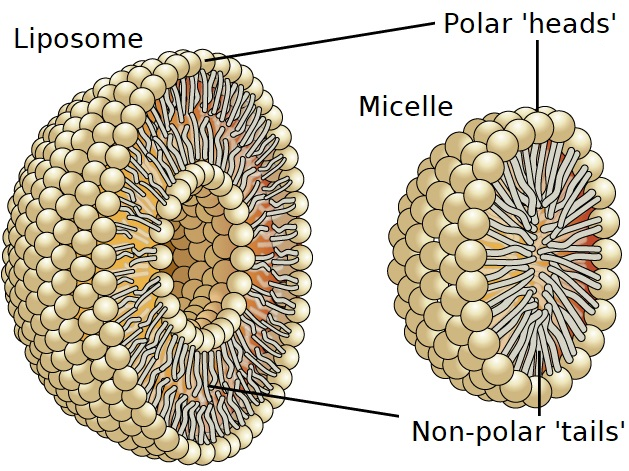
\includegraphics{figures/ch3/OSC_Microbio_07_03_micelle_edit.png}

}

}

\end{minipage}%
%
\begin{minipage}[t]{0.01\linewidth}

{\centering 

~

}

\end{minipage}%
%
\begin{minipage}[t]{0.03\linewidth}

{\centering 

\raisebox{-\height}{


\includegraphics{figures/(b).png}

}

}

\end{minipage}%
%
\begin{minipage}[t]{0.01\linewidth}

{\centering 

~

}

\end{minipage}%
%
\begin{minipage}[t]{0.36\linewidth}

{\centering 

\raisebox{-\height}{

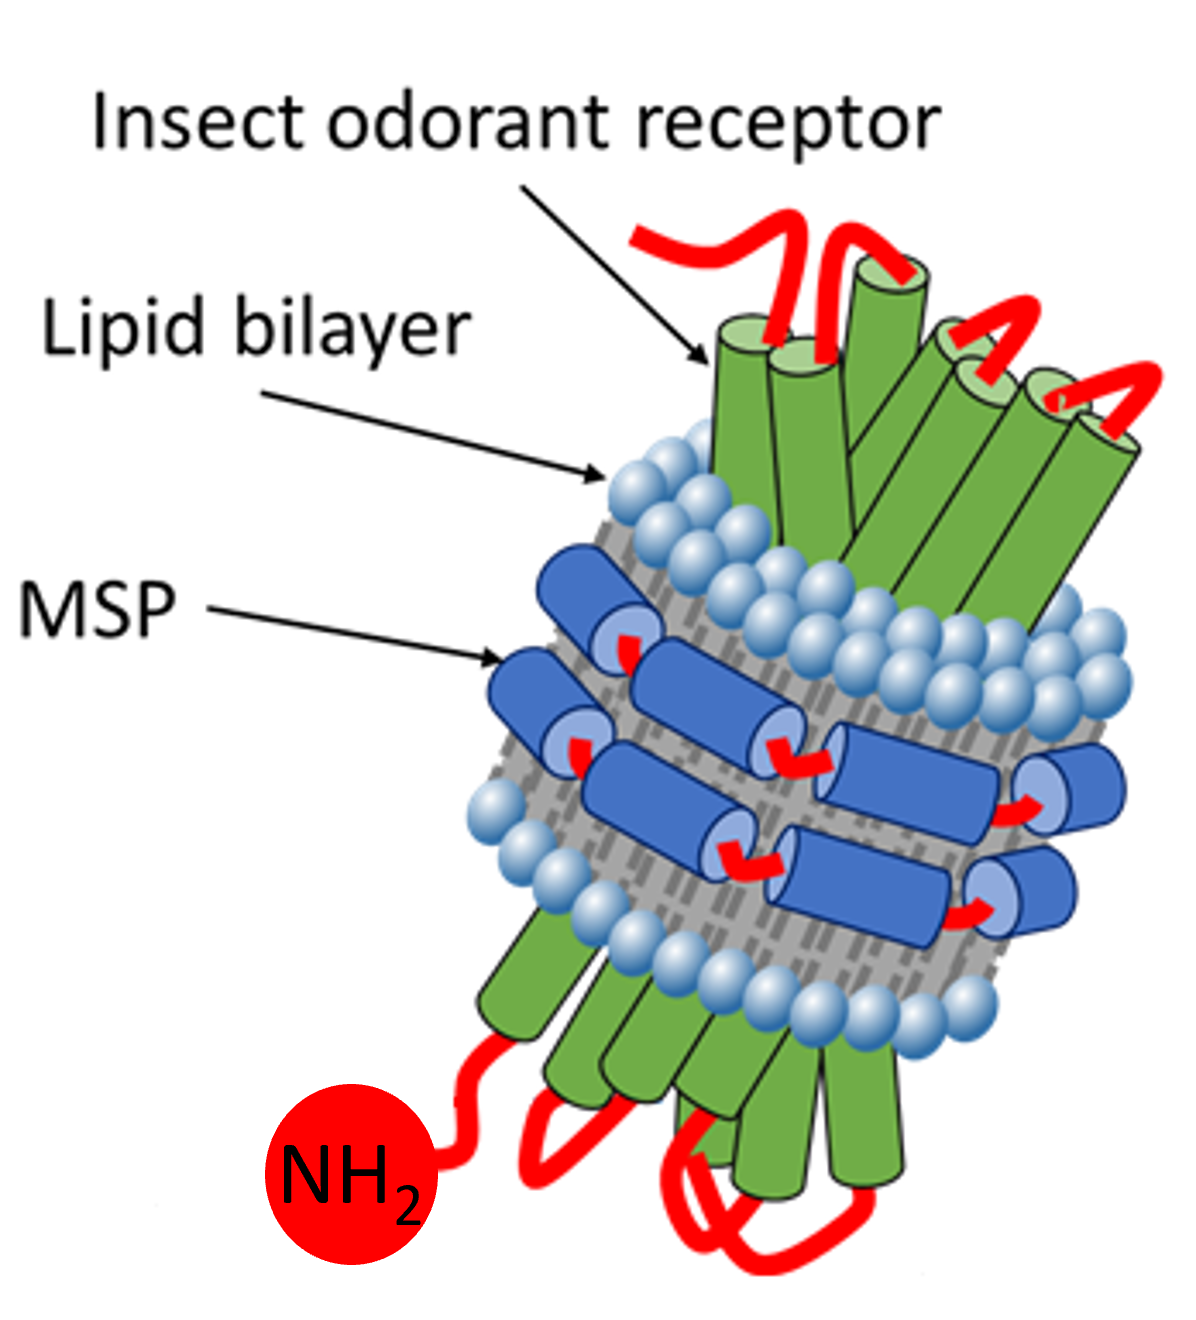
\includegraphics{figures/ch3/iOR_nanodisc.png}

}

}

\end{minipage}%
%
\begin{minipage}[t]{0.01\linewidth}

{\centering 

~

}

\end{minipage}%

\caption[Diagrams showing the structure of various artificial
membranes.]{\label{fig-membranes}Liposomes and micelles are shown in (a)
with the hydrophilic heads and hydrophobic tails indicated. A lipid
nanodisc wrapped around an insect odorant receptor transmembrane protein
is shown in (b), where the amine group shown is the odorant receptor
N-terminus. The nanodisc consists of a lipid bilayer encircled by a
membrane scaffold protein (MSP). Images are not to scale. The schematic
in (a) is adapted from \autocite{Micelle}, and used under the CC BY-4.0
license. The schematic in (b) is reprinted with permission from
\autocite{Murugathas2019a}. Copyright \(\copyright\) 2019 American
Chemical Society.}

\end{figure}

A nanovesicle is a nanoscopic spherical bilayer fluid sac. There are
various types of artificial nanovesicles, including liposomes,
ethosomes, transfersomes, niosomes and phytosomes. The type of
nanovesicle depends on its chemical makeup \autocite{Ramadon2022}. For
example, a liposome is made up of phospholipid and cholesterol, and can
consist of one or more concentric amphiphilic bilayers. The liposome can
contain hydrophobic compounds within the bilayer due to hydrophobic
interactions, while hydrophilic compounds are held within the vesicle
core or interior \autocite{Nath2007,Ramadon2022}. A nanovesicle can be
used solely as a format to protect membrane proteins
\autocite{Murugathas2020}, or with the addition of integrated ion
channels, can mimic the operation of a cell \emph{in vivo}, with
intracellular signalling pathways triggered by the membrane proteins
\autocite{Lim2015}. Nanomicelles (or simply micelles) are also
nanoscopic and spherical, but unlike nanovesicles, they have no inner
fluid sac \autocite{Nath2007,Bose2021}. Micelles self-assemble when
phospholipid is mixed with detergent. The surface of the micelle is made
up of the hydrophilic detergent and phospholipid heads, while the
internal core is made up of the hydrophobic phospholipid tail
\autocite{Nath2007}. Hydrophobic compounds can be contained within the
core of the micelle \autocite{Bose2021}. Figure~\ref{fig-membranes} (a)
illustrates the difference between the liposome and micelle structures.

Nanodiscs have emerged as a model membrane candidate with many
advantages over the more traditional nanovesicle and micelle formats.
The nanodisc is a disc-shaped lipid bilayer encompassed by an membrane
scaffold protein (MSP), with structure pictured in
Figure~\ref{fig-membranes} (b) \autocite{Nath2007,Bayburt2010,Yang2018}.
The amphiphilic membrane scaffold protein protects the exposed, strongly
hydrophobic side chains of the nanodisc in an aqueous environment
\autocite{Fruh2011,Yang2018}. Unlike liposomes and micelles, there is
little variation between the size of individual nanodiscs due to
constraints placed on the bilayer by the encompassing scaffold protein
used, meaning greater consistency within and between membrane batches
\autocite{Nath2007,Fruh2011}. Nanodiscs have also been found to be
significantly less prone to non-specific binding (see
Section~\ref{sec-non-specific-binding}) than micelles
\autocite{Fruh2011}. Another advantage of nanodiscs is that the membrane
scaffold protein can be attached to biosensor surfaces at specific
affinity tags, for example, the scaffold protein hexahistidine tag
(his-tag) \autocite{Bayburt2010,Fruh2011}. Depending on the type of MSP
used, a nanodisc measures between \(10 - 20\) nm across and can hold
either a single receptor or several odorant receptors
\autocite{Nath2007,Bayburt2010}. Furthermore, the protein coating of the
nanodisc makes it particularly stable. The stability of nanodiscs means
they can be used to produce particularly reliable and long-lived
biosensor devices \autocite{Goldsmith2011,Yang2018,Moon2020,Cheema2021}.

\hypertarget{sec-sensor-types}{%
\subsection{Sensor Functionalisation}\label{sec-sensor-types}}

Table~\ref{tbl-or-biosensors} summarises all published odorant receptor
functionalised carbon nanotube and graphene field-effect
transistor-based sensors to date. The majority of published works on
this topic come from the Tai Hyun Park group at Seoul National
University. The Park group has mainly focused on CNT FETs functionalised
with human odorant receptors, but has used a range of different
transducer immobilisation techniques when producing the sensors.

\newgeometry{a4paper,centering=true,right=1.5in,headsep=44.95pt,footskip=23pt}
\begin{landscape}
\begin{center}

\hypertarget{tbl-or-biosensors}{}
\begin{longtable}[]{@{}lllllll@{}}
\caption{\label{tbl-or-biosensors}Summary of past fabrication methods
for odorant receptor-functionalised thin-film transistor
biosensors.}\tabularnewline
\toprule\noalign{}
Attachment & Attachment Method & References & Transducer & OR Type & OR
Format & LOD \\
\midrule\noalign{}
\endfirsthead
\toprule\noalign{}
Attachment & Attachment Method & References & Transducer & OR Type & OR
Format & LOD \\
\midrule\noalign{}
\endhead
\bottomrule\noalign{}
\endlastfoot
Non-covalent & Vacuum-drying & Kim, 2009. \cite{Kim2009a} & CNTFET &
Human & Cell membrane & 100 fM \\
& DMT-MM & Yoon, 2009. \cite{Yoon2009} & CNTFET & Human & Cell membrane
& 10 fM \\
& PDL & Jin, 2012. \cite{Jin2012} & CNTFET & Human & Nanovesicles & 1
fM \\
& & Park, 2012. \cite{Park2012a} & CNTFET & Dog & Nanovesicles & 1 fM \\
& & Lim, 2015. \cite{Lim2015} & CNTFET & Human & Nanovesicles & 1 fM \\
& & Son, 2015. \cite{Son2015} & CNTFET & Human & Nanovesicles & 10
ng/L \\
& & Ahn, 2015. \cite{Ahn2015} & CNTFET & Human & Nanovesicles & 1 fM \\
& GA-conjugated DAN & Park, 2012. \cite{Park2012} & GFET & Human & Cell
membrane & 0.04 fM \\
& & Lee, 2012. \cite{Lee2012b} & CNTFET & Human & Cell membrane & 1
fM \\
& & Kwon, 2015. \cite{Kwon2015} & GFET & Human & Cell membrane & 0.1
fM \\
& & Goodwin, 2021. \cite{Goodwin2021} & GFET & Human & Cell membrane &
0.5 pM \\
& PBASE & Murugathas, 2019. \cite{Murugathas2019a} & CNTFET &
\textit{Insect} & Nanodiscs & 1 fM \\
& & Murugathas, 2020. \cite{Murugathas2020} & GFET & \textit{Insect} &
Nanovesicles, Nanodiscs & 1 fM \\
& & Ahn, 2020. \cite{Ahn2020} & GFET & Human & Nanovesicles & 100 fM \\
& & Yoo, 2022. \cite{Yoo2022} & CNTFET & Human & Micelles & 1 fM \\
Covalent & Diazonium salt/Ni-NTA & Goldsmith, 2011. \cite{Goldsmith2011}
& CNTFET & Mouse & Micelles, Nanodiscs & \textasciitilde7 ppb \\
& & Son, 2017. \cite{Son2017} & CNTFET & Human & Micelles & 10 fM \\
& Half-v5 mouse Ab & Lee, 2018. \cite{Lee2018} & CNTFET & Human &
Nanodiscs & 1 fM \\
\end{longtable}

\end{center}
\end{landscape}
\restoregeometry % Restore the global document page margins

Dog and mouse odorant receptors have also been used with carbon nanotube
and graphene field-effect transducers in bioelectronic nose
applications, by the Park group and by Goldsmith \emph{et al.}
respectively. As far as the author knows, the Plank group at Te Herenga
Waka \(-\) Victoria University of Wellington is the only group to have
produced thin-film transistors functionalised with insect odorant
receptors. The behaviour of insect odorant receptors is significantly
different to that of vertebrate odorant receptors, and their behaviour
in sensor applications is currently not well understood. The distinction
between vertebrate and insect odorant receptors is discussed in more
depth in Section~\ref{sec-insect-OR-biosensors}.

For a bioelectronic nose to operate, sufficient coupling must exist
between the bioreceptor element and the graphene or carbon nanotube
channel of the field-effect transistor. Odorant receptors can be
directly attached by physical adsorption; however, this approach is
difficult to control, and can lead to weak coupling between the odorant
receptors and the transducer \autocite{Kwon2015,Dung2018,Bohbot2020}.
Alternatively, a bifunctional linker element may mediate the attachment
between functional groups of the bioreceptor and the transducer in a
biochemical process referred to as ``functionalisation''
\autocite{Star2003a}. Functionalisation may involve covalent or
non-covalent bonding to the carbon-ring transducer surface. Covalent
bonding is stronger than non-covalent bonding, and therefore gives a
more permanent attachment between linker molecules and the transducer.

Unlike covalent attachment, non-covalent attachment preserves the
polycyclic \(sp^2\) bonding of carbon atoms in graphene and carbon
nanotubes and therefore the electrical properties of the channel
\autocite{DiCrescenzo2014,Yao2021,Shkodra2021,Li2023}. For example, one
group found covalent bonding of diazonium linker caused a \(\sim 50\) \%
drop in graphene channel mobility \autocite{Lerner2014}. In comparison,
only a \(\sim 5\) \% drop in mobility was seen for attachment of a
mixture of linkers containing pyrene to a graphene channel via
non-covalent pi-stacking \autocite{Thodkar2021}. The relative advantages
and disadvantages of each type of receptor immobilisation can be found
in Table~\ref{tbl-functionalisation-types}.

\hypertarget{tbl-functionalisation-types}{}
\begin{longtable}[t]{>{\raggedright\arraybackslash}p{5.4cm}>{\raggedright\arraybackslash}p{1.45cm}>{\raggedright\arraybackslash}p{1.3cm}>{\raggedright\arraybackslash}p{1.45cm}>{\raggedright\arraybackslash}p{1.3cm}>{\raggedright\arraybackslash}p{1.3cm}}
\caption{\label{tbl-functionalisation-types}A comparison of the advantages and disadvantages of different approaches
for immobilising odorant receptors onto thin-film transducers. }\tabularnewline

\toprule
Attachment Type & Simplicity & Synergy & Specificity & Stability & Strength\\
\midrule
Direct Adsorption & High & Medium & Low & Low & Low\\
Linker, covalently tethered & Medium & Low & High & High & High\\
Linker, non-covalently tethered & Medium & High & Medium & Medium & Medium\\
\bottomrule
\end{longtable}

Three functionalisation linkers were used by both the Park group and a
secondary research group: non-covalently attached glutaraldehyde
(GA)-conjugated 1,5-diaminonaphthalene (DAN)
\autocite{Kwon2015,Goodwin2021}, non-covalently attached
1-pyrenebutanoic acid N-hydroxysuccinimide ester (PBASE)
\autocite{Murugathas2020,Yoo2022}, and covalently attached
nickel-nitrilotriacetic acid (Ni-NTA) modified diazonium salt
\autocite{Goldsmith2011,Son2017}. The bonding between the linker
molecule and receptor element is typically covalent, regardless of the
type of bonding that exists between linker and transducer.
Interestingly, no single paper compares multiple possible
functionalisation techniques directly, making it difficult to assess the
relative quality of various attachment methods. The limit of detection
(LOD) could be used as a rough measure of quality. The functionalisation
procedure resulting in the lowest limit of detection used was
non-covalent \autocite{Park2012}. However, the quoted LOD is highly
variable across the non-covalently functionalised devices. Furthermore,
non-covalent functionalisation of odorant receptors has never been used
for vapour sensing. The next section further explores the sensing
behaviour of biosensors functionalised with the most commonly-used
protocols.

\hypertarget{sec-biosensor-methods}{%
\subsection{Sensing Behaviour}\label{sec-biosensor-methods}}

\begin{figure}

\begin{minipage}[t]{0.03\linewidth}

{\centering 

\raisebox{-\height}{


\includegraphics{figures/(a).png}

}

}

\end{minipage}%
%
\begin{minipage}[t]{0.01\linewidth}

{\centering 

~

}

\end{minipage}%
%
\begin{minipage}[t]{0.45\linewidth}

{\centering 

\raisebox{-\height}{

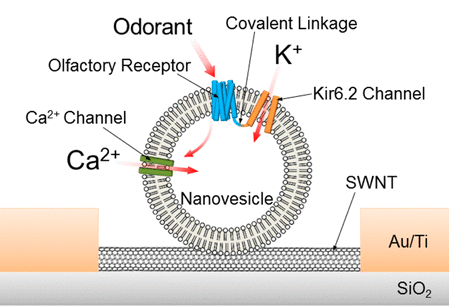
\includegraphics{figures/ch3/ion-channel-nanovesicle-lim2015.png}

}

}

\end{minipage}%
%
\begin{minipage}[t]{0.01\linewidth}

{\centering 

~

}

\end{minipage}%
%
\begin{minipage}[t]{0.03\linewidth}

{\centering 

\raisebox{-\height}{


\includegraphics{figures/(b).png}

}

}

\end{minipage}%
%
\begin{minipage}[t]{0.01\linewidth}

{\centering 

~

}

\end{minipage}%
%
\begin{minipage}[t]{0.45\linewidth}

{\centering 

\raisebox{-\height}{

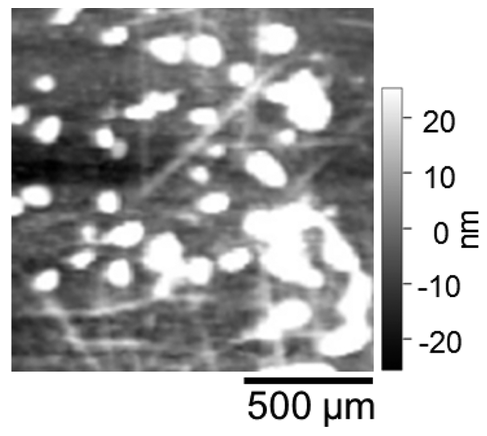
\includegraphics{figures/ch3/afm-nanovesicle-lim2015.png}

}

}

\end{minipage}%
%
\begin{minipage}[t]{0.01\linewidth}

{\centering 

~

}

\end{minipage}%
\newline
\begin{minipage}[t]{0.03\linewidth}

{\centering 

\raisebox{-\height}{


\includegraphics{figures/(c).png}

}

}

\end{minipage}%
%
\begin{minipage}[t]{0.01\linewidth}

{\centering 

~

}

\end{minipage}%
%
\begin{minipage}[t]{0.45\linewidth}

{\centering 

\raisebox{-\height}{

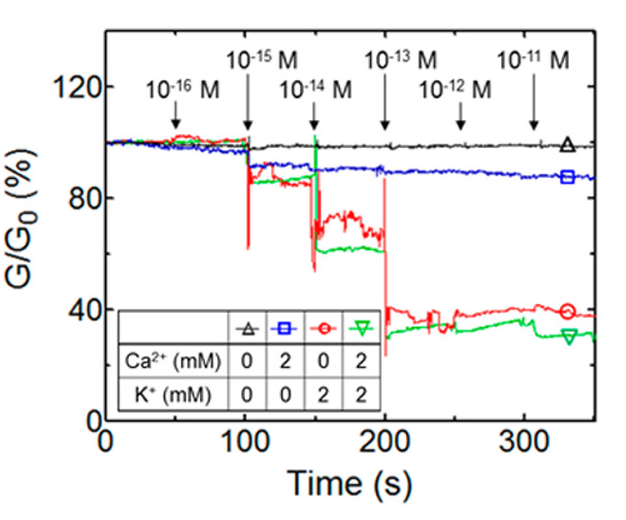
\includegraphics{figures/ch3/nanovesicle-amyl-butyrate-1-lim2015.png}

}

}

\end{minipage}%
%
\begin{minipage}[t]{0.01\linewidth}

{\centering 

~

}

\end{minipage}%
%
\begin{minipage}[t]{0.03\linewidth}

{\centering 

\raisebox{-\height}{


\includegraphics{figures/(d).png}

}

}

\end{minipage}%
%
\begin{minipage}[t]{0.01\linewidth}

{\centering 

~

}

\end{minipage}%
%
\begin{minipage}[t]{0.45\linewidth}

{\centering 

\raisebox{-\height}{

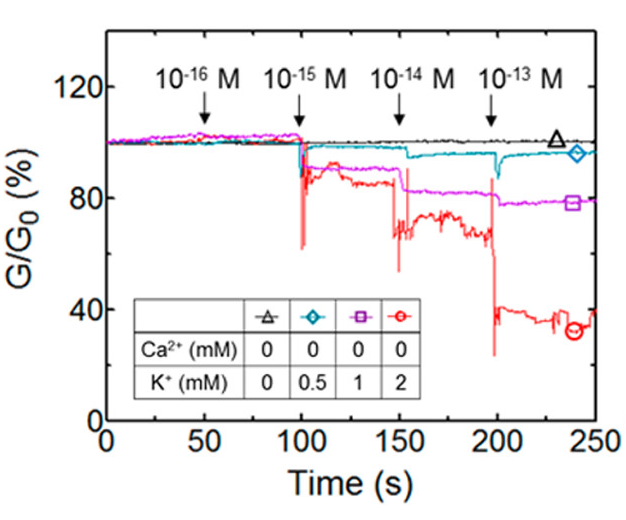
\includegraphics{figures/ch3/lim2015-potassium1.png}

}

}

\end{minipage}%
%
\begin{minipage}[t]{0.01\linewidth}

{\centering 

~

}

\end{minipage}%
\newline
\begin{minipage}[t]{0.03\linewidth}

{\centering 

\raisebox{-\height}{


\includegraphics{figures/(e).png}

}

}

\end{minipage}%
%
\begin{minipage}[t]{0.01\linewidth}

{\centering 

~

}

\end{minipage}%
%
\begin{minipage}[t]{0.45\linewidth}

{\centering 

\raisebox{-\height}{

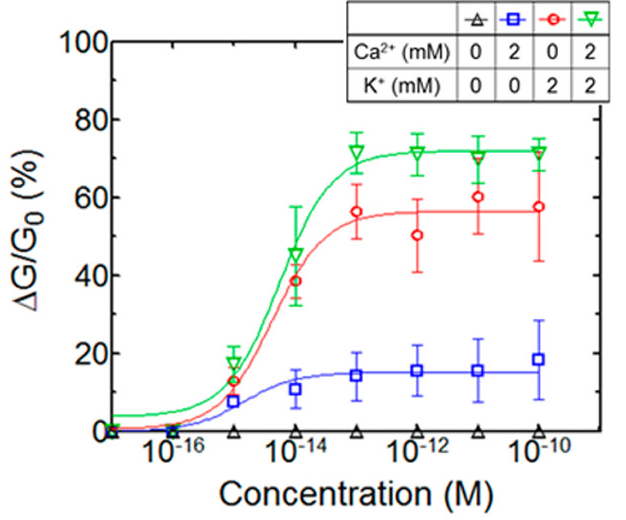
\includegraphics{figures/ch3/nanovesicle-amyl-butyrate-2-lim2015.png}

}

}

\end{minipage}%
%
\begin{minipage}[t]{0.01\linewidth}

{\centering 

~

}

\end{minipage}%
%
\begin{minipage}[t]{0.03\linewidth}

{\centering 

\raisebox{-\height}{


\includegraphics{figures/(f).png}

}

}

\end{minipage}%
%
\begin{minipage}[t]{0.01\linewidth}

{\centering 

~

}

\end{minipage}%
%
\begin{minipage}[t]{0.45\linewidth}

{\centering 

\raisebox{-\height}{

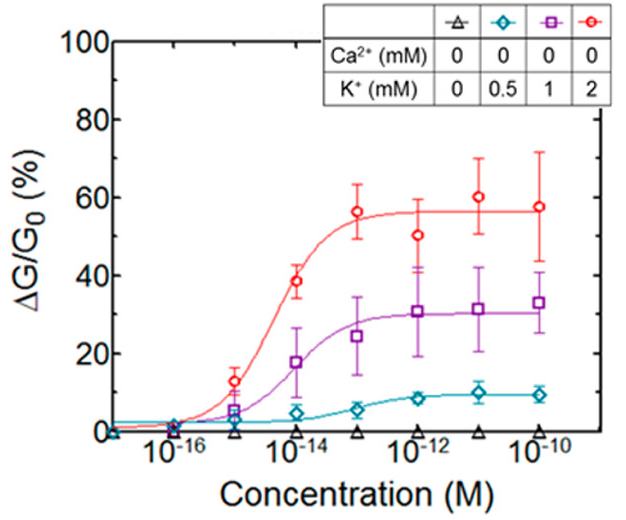
\includegraphics{figures/ch3/lim2015-potassium2.png}

}

}

\end{minipage}%
%
\begin{minipage}[t]{0.01\linewidth}

{\centering 

~

}

\end{minipage}%

\caption[Schematics detailing the nanovesicle-based carbon nanotube
field-effect biosensor of Lim \emph{et
al.}]{\label{fig-lim-ion-channel}Schematics detailing the
nanovesicle-based carbon nanotube field-effect biosensor of Lim \emph{et
al.} (a) shows a schematic of the various signalling pathways present in
the sensor (not to scale), while (b) shows an atomic force microscope
image of the functionalised device. Real-time conductance changes
resulting from amyl butyrate additions are compared against relevant
controls in (c) and (d), while the dose-dependent response patterns to
amyl butyrate corresponding to (c) and (d) are shown in (e) and (f)
respectively. The key in (c)-(f) indicates the concentration of ions
available to flow through nanovesicle ion channels in each experimental
series. Reprinted with permission from \autocite{Lim2015}. Copyright
\(\copyright\) 2015 American Chemical Society.}

\end{figure}

\begin{figure}

\begin{minipage}[t]{0.03\linewidth}

{\centering 

\raisebox{-\height}{


\includegraphics{figures/(a).png}

}

}

\end{minipage}%
%
\begin{minipage}[t]{0.04\linewidth}

{\centering 

~

}

\end{minipage}%
%
\begin{minipage}[t]{0.90\linewidth}

{\centering 

\raisebox{-\height}{

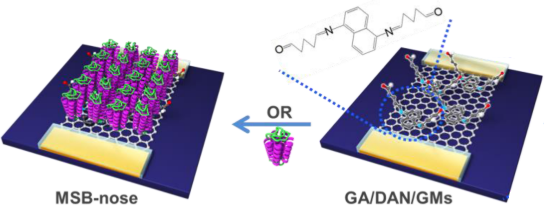
\includegraphics{figures/ch3/kwon2015-OR-graphene.png}

}

}

\end{minipage}%
%
\begin{minipage}[t]{0.04\linewidth}

{\centering 

~

}

\end{minipage}%
\newline
\begin{minipage}[t]{0.03\linewidth}

{\centering 

\raisebox{-\height}{


\includegraphics{figures/(b).png}

}

}

\end{minipage}%
%
\begin{minipage}[t]{0.01\linewidth}

{\centering 

~

}

\end{minipage}%
%
\begin{minipage}[t]{0.45\linewidth}

{\centering 

\raisebox{-\height}{

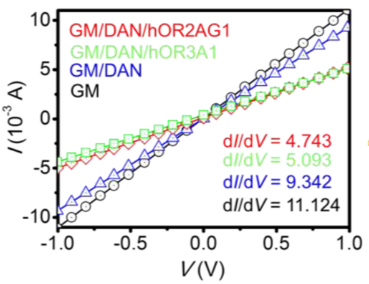
\includegraphics{figures/ch3/kwon2015_transfer.png}

}

}

\end{minipage}%
%
\begin{minipage}[t]{0.01\linewidth}

{\centering 

~

}

\end{minipage}%
%
\begin{minipage}[t]{0.03\linewidth}

{\centering 

\raisebox{-\height}{


\includegraphics{figures/(c).png}

}

}

\end{minipage}%
%
\begin{minipage}[t]{0.01\linewidth}

{\centering 

~

}

\end{minipage}%
%
\begin{minipage}[t]{0.45\linewidth}

{\centering 

\raisebox{-\height}{

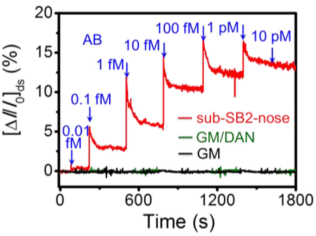
\includegraphics{figures/ch3/kwon2015-amyl-butyrate.png}

}

}

\end{minipage}%
%
\begin{minipage}[t]{0.01\linewidth}

{\centering 

~

}

\end{minipage}%
\newline
\begin{minipage}[t]{0.03\linewidth}

{\centering 

\raisebox{-\height}{


\includegraphics{figures/(d).png}

}

}

\end{minipage}%
%
\begin{minipage}[t]{0.01\linewidth}

{\centering 

~

}

\end{minipage}%
%
\begin{minipage}[t]{0.45\linewidth}

{\centering 

\raisebox{-\height}{

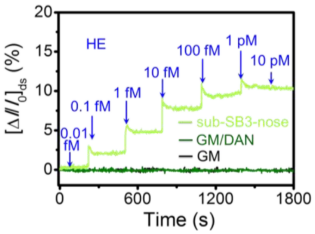
\includegraphics{figures/ch3/kwon2015-helional.png}

}

}

\end{minipage}%
%
\begin{minipage}[t]{0.01\linewidth}

{\centering 

~

}

\end{minipage}%
%
\begin{minipage}[t]{0.03\linewidth}

{\centering 

\raisebox{-\height}{


\includegraphics{figures/(e).png}

}

}

\end{minipage}%
%
\begin{minipage}[t]{0.01\linewidth}

{\centering 

~

}

\end{minipage}%
%
\begin{minipage}[t]{0.45\linewidth}

{\centering 

\raisebox{-\height}{

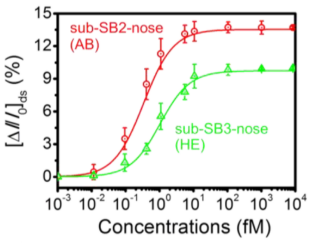
\includegraphics{figures/ch3/kwon2015-dose.png}

}

}

\end{minipage}%
%
\begin{minipage}[t]{0.01\linewidth}

{\centering 

~

}

\end{minipage}%

\caption[Schematics showing the odorant receptor-functionalised graphene
field-effect biosensor of Kwon \emph{et
al.}]{\label{fig-kwon-multiplexed}Schematics showing the odorant
receptor-functionalised graphene field-effect biosensor of Kwon \emph{et
al.} (a) shows the functionalisation of odorant receptors onto graphene
using non-covalently attached GA-modified DAN linker; (b) compares
transfer characteristics of the device with graphene only (GM), graphene
with DAN linker (GM/DAN), and after modification with one of two
different ORs (hOR2AG1, hOR3A1); (c) shows the real-time responses of
the liquid-gated hOR2AG1-modified transistor (sub-SB2) to various
concentrations of amyl butyrate (AB) analyte; (d) shows the real-time
responses of the hOR3A1-modified transistor (sub-SB3) to various
concentrations of helional (HE) analyte; and (e) shows the
dose-dependent response curve corresponding to the sub-SB2 and sub-SB3
sensors. Reprinted with permission from \autocite{Kwon2015}. Copyright
\(\copyright\) 2015 American Chemical Society.}

\end{figure}

\begin{figure}

\begin{minipage}[t]{0.03\linewidth}

{\centering 

\raisebox{-\height}{


\includegraphics{figures/(a).png}

}

}

\end{minipage}%
%
\begin{minipage}[t]{0.01\linewidth}

{\centering 

~

}

\end{minipage}%
%
\begin{minipage}[t]{0.45\linewidth}

{\centering 

\raisebox{-\height}{

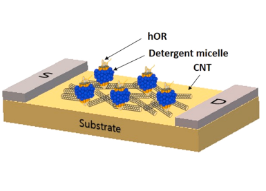
\includegraphics{figures/ch3/yoo2022-micelle-cnt.png}

}

}

\end{minipage}%
%
\begin{minipage}[t]{0.01\linewidth}

{\centering 

~

}

\end{minipage}%
%
\begin{minipage}[t]{0.03\linewidth}

{\centering 

\raisebox{-\height}{


\includegraphics{figures/(b).png}

}

}

\end{minipage}%
%
\begin{minipage}[t]{0.01\linewidth}

{\centering 

~

}

\end{minipage}%
%
\begin{minipage}[t]{0.45\linewidth}

{\centering 

\raisebox{-\height}{

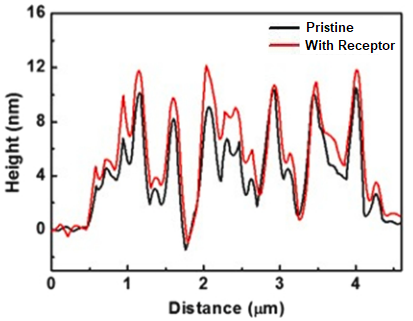
\includegraphics{figures/ch3/yoo2022-AFM.png}

}

}

\end{minipage}%
%
\begin{minipage}[t]{0.01\linewidth}

{\centering 

~

}

\end{minipage}%
\newline
\begin{minipage}[t]{0.03\linewidth}

{\centering 

\raisebox{-\height}{


\includegraphics{figures/(c).png}

}

}

\end{minipage}%
%
\begin{minipage}[t]{0.01\linewidth}

{\centering 

~

}

\end{minipage}%
%
\begin{minipage}[t]{0.45\linewidth}

{\centering 

\raisebox{-\height}{

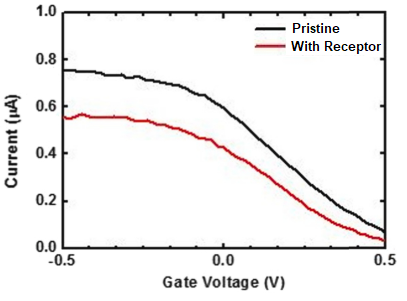
\includegraphics{figures/ch3/yoo2022-TX.png}

}

}

\end{minipage}%
%
\begin{minipage}[t]{0.01\linewidth}

{\centering 

~

}

\end{minipage}%
%
\begin{minipage}[t]{0.03\linewidth}

{\centering 

\raisebox{-\height}{


\includegraphics{figures/(d).png}

}

}

\end{minipage}%
%
\begin{minipage}[t]{0.01\linewidth}

{\centering 

~

}

\end{minipage}%
%
\begin{minipage}[t]{0.45\linewidth}

{\centering 

\raisebox{-\height}{

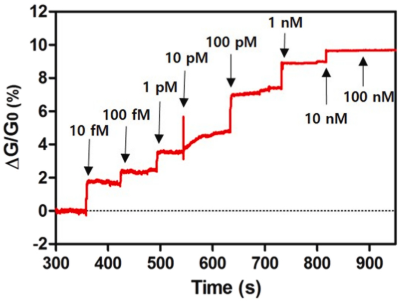
\includegraphics{figures/ch3/yoo2022-DMMP.png}

}

}

\end{minipage}%
%
\begin{minipage}[t]{0.01\linewidth}

{\centering 

~

}

\end{minipage}%
\newline
\begin{minipage}[t]{0.03\linewidth}

{\centering 

\raisebox{-\height}{


\includegraphics{figures/(e).png}

}

}

\end{minipage}%
%
\begin{minipage}[t]{0.01\linewidth}

{\centering 

~

}

\end{minipage}%
%
\begin{minipage}[t]{0.45\linewidth}

{\centering 

\raisebox{-\height}{

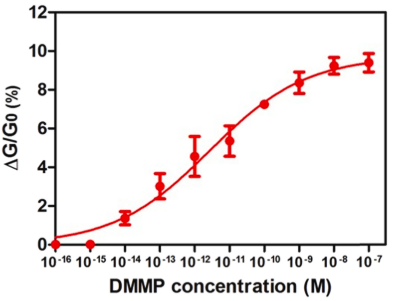
\includegraphics{figures/ch3/yoo2022-DMMP-2.png}

}

}

\end{minipage}%
%
\begin{minipage}[t]{0.01\linewidth}

{\centering 

~

}

\end{minipage}%
%
\begin{minipage}[t]{0.03\linewidth}

{\centering 

\raisebox{-\height}{


\includegraphics{figures/(f).png}

}

}

\end{minipage}%
%
\begin{minipage}[t]{0.01\linewidth}

{\centering 

~

}

\end{minipage}%
%
\begin{minipage}[t]{0.45\linewidth}

{\centering 

\raisebox{-\height}{

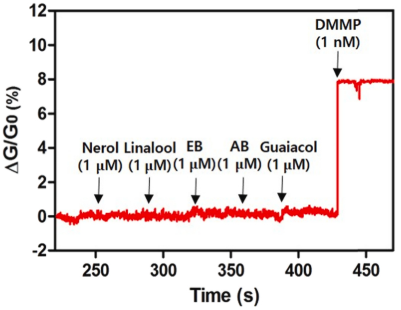
\includegraphics{figures/ch3/yoo2022-DMMP-3.png}

}

}

\end{minipage}%
%
\begin{minipage}[t]{0.01\linewidth}

{\centering 

~

}

\end{minipage}%

\caption[Schematics of the micelle-based carbon nanotube field-effect
transistor of Yoo \emph{et al.}]{\label{fig-yoo-micelle}Schematics of
the micelle-based carbon nanotube field-effect transistor of Yoo
\emph{et al.} (a) shows the functionalisation of detergent micelles onto
the carbon nanotube network channel; (b) shows the same height profile
across an atomic force microscope image of the carbon nanotube network
before and after functionalisation with micelles using PBASE; (c) shows
the liquid-gated transfer characteristic of a device channel before and
after functionalisation with PBASE and micelles; (d) shows real-time
responses of the functionalised, liquid-gated channel to additions of
dimethyl methylphosphonate (DMMP) analyte; (e) shows the dose-dependent
response curve to DMMP; and (f) shows a control series demonstrating the
selective behaviour of the sensor (EB is ethyl butyrate, AB is amyl
butyrate). Adapted with permission from \autocite{Yoo2022}. Copyright
\(\copyright\) 2022 Elsevier.}

\end{figure}

Vertebrate odorant receptors have previously been coupled with
nanovesicle ion channels for selective analyte detection
\autocite{Lim2015,Dung2018}. Lim \emph{et al.} synthesised nanovesicles
featuring the human odorant receptor hOR2AG1, covalently coupled with a
potassium ion channel and placed alongside an endogenous calcium ion
channel. This configuration is shown in Figure~\ref{fig-lim-ion-channel}
(a). These nanovesicles were attached to the carbon nanotube network of
a thin-film device via charge-charge interaction with poly-D-lysine,
demonstrated with the atomic force microscope image in
Figure~\ref{fig-lim-ion-channel} (b). Binding of amyl butyrate to
hOR2AG1 causes the OR to change conformation, opening the coupled
potassium ion channel and causing ions to flow into the nanovesicle,
resulting in transistor channel gating. The real-time signal responses
associated with channel gating due to ion flow are shown in
Figure~\ref{fig-lim-ion-channel} (c)-(f). Intracellular signalling by
the odorant receptors means that target binding also activates the
calcium ion channel, and so the presence of calcium ions is sufficient
for a sensing response. In all electrolytes used to obtain a signal
response, ions are present in high concentrations relative to analyte,
ensuring ions are readily available for signalling processes. Without
either potassium or calcium ions present, ion inflow cannot occur, so no
conductance change is observed \autocite{Lim2015}.

Odorant receptors can also be expressed in the native cell membrane and
attached directly to the biosensor channel. Here, the changes in odorant
receptor conformation that result from analyte binding cause affects the
distance between charges on the odorant receptor and the transducer
channel, gating the channel \autocite{Kwon2015,Dung2018}. Kwon \emph{et
al.} functionalised graphene field-effect transistors with human odorant
receptors hOR2AG1 and hOR3A1 using non-covalently attached
1,5-diaminonaphthalene (DAN) modified with glutaraldehyde (GA) as a
linker, as shown in Figure~\ref{fig-kwon-multiplexed} (a). The odorant
receptors attach to the GA-modified DAN via a Schiff-base reaction
\autocite{Bhatt2021}. OR attachment was demonstrated by SEM imaging as
well as a significant change in device resistance, shown in
Figure~\ref{fig-kwon-multiplexed} (b). Both hOR2AG1 and hOR3A1 showed
real-time responses to their corresponding target analyte at
sub-femtomolar concentrations, as shown in
Figure~\ref{fig-kwon-multiplexed} (c) and
Figure~\ref{fig-kwon-multiplexed} (d) respectively. No responses were
seen from linker-modified graphene to the same analyte additions. The
dose-dependent response curve of both these odorant receptor sensors is
shown in Figure~\ref{fig-kwon-multiplexed} (e). As in
Figure~\ref{fig-lim-ion-channel} (d), the response behaviour follows a
curve which can be described using a Langmuir surface adsorption
isotherm, with saturation behaviour observed with picomolar additions.

Biosensors have also been produced where odorant receptors are held in a
detergent micelle format instead of the native cell membrane. The
mechanism behind sensing is the same as for odorant receptors in the
cell membrane, where a conformational change in the odorant receptors
leads to channel gating \autocite{Dung2018,Yoo2022}. Yoo \emph{et al.}
functionalised random-network CNT FETs with detergent micelles which
contained human odorant receptor hOR2T7. PBASE was used as the linker
molecule, which attaches to the odorant receptor via its amine group and
non-covalently tethers it to the transducer, illustrated in
Figure~\ref{fig-yoo-micelle} (a). Successful immobilisation was
demonstrated by a raised atomic force microscope height profile after
receptor attachment (Figure~\ref{fig-yoo-micelle} (b)) and an on-current
drop in the liquid-gated transfer characteristics of the device
(Figure~\ref{fig-yoo-micelle} (c)). The sensor showed sharp real-time
responses to the addition of DMMP concentrations, as seen in
Figure~\ref{fig-yoo-micelle} (d). The dose dependence curve for DMMP
responses is shown in in Figure~\ref{fig-yoo-micelle} (e), again showing
a Langmuir-type response curve to successive DMMP additions. Various
analytes with a similar scent to DMMP were added at high concentrations
to the liquid-gate, shown in Figure~\ref{fig-yoo-micelle} (f). No
response was seen to any these additions, demonstrating the selectivity
of the sensor.

\begin{figure}

\begin{minipage}[t]{0.03\linewidth}

{\centering 

\raisebox{-\height}{


\includegraphics{figures/(a).png}

}

}

\end{minipage}%
%
\begin{minipage}[t]{0.01\linewidth}

{\centering 

~

}

\end{minipage}%
%
\begin{minipage}[t]{0.40\linewidth}

{\centering 

\raisebox{-\height}{

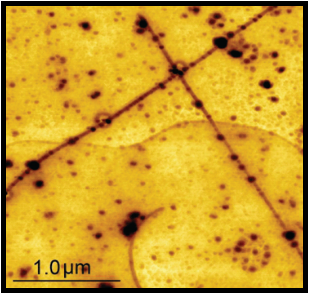
\includegraphics{figures/ch3/afm-nanodisc-goldsmith.png}

}

}

\end{minipage}%
%
\begin{minipage}[t]{0.01\linewidth}

{\centering 

~

}

\end{minipage}%
%
\begin{minipage}[t]{0.03\linewidth}

{\centering 

\raisebox{-\height}{


\includegraphics{figures/(b).png}

}

}

\end{minipage}%
%
\begin{minipage}[t]{0.01\linewidth}

{\centering 

~

}

\end{minipage}%
%
\begin{minipage}[t]{0.50\linewidth}

{\centering 

\raisebox{-\height}{

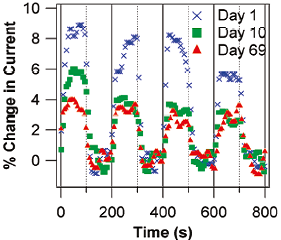
\includegraphics{figures/ch3/eugenol-goldsmith.png}

}

}

\end{minipage}%
%
\begin{minipage}[t]{0.01\linewidth}

{\centering 

~

}

\end{minipage}%

\caption[Functionalisation and sensing behaviour of the nanodisc-based
carbon nanotube field-effect transistor of Goldsmith \emph{et
al.}]{\label{fig-eugenol-responses}The functionalisation of mOR174-9
nanodiscs onto single-CNT field effect transistor vapour sensing use is
demonstrated with an atomic force microscope image in (a), while (b)
shows real-time responses of the sensor to 2 ppm eugenol vapour. The
response to eugenol on day 69 (red triangles) indicates that the device
retains the ability to respond to eugenol 10 weeks after
functionalisation. Reprinted with permission from
\autocite{Goldsmith2011}. Copyright \(\copyright\) 2011 American
Chemical Society.}

\end{figure}

In the first study of its kind, Goldsmith \emph{et al.} demonstrated
that a single-CNT device functionalised with mOR174-9 odorant receptors
in either a micelle or nanodisc format could be used as a vapour-phase
biosensor. Micelle immobilisation was confirmed using atomic force
microscopy, as shown in Figure~\ref{fig-eugenol-responses} (a). The mOR
CNT FETs were exposed to nitrogen flow at 50\% relative humidity. The
conductance across the channel was measured while a specific
concentration of the positive ligand eugenol was added to the constant
flow for 100 s, then removed from the flow for 100 s. This cycle was
repeated five times. Figure~\ref{fig-eugenol-responses} (b) shows that a
\(\sim\) 9\% increase in current was observed during each cycle of
exposure to eugenol. The device still responded to eugenol cycles after
69 days of storage in 25\% (v/v) ethanol at 4 °C. This persistent
activity may result from the long-lived nanodisc format used
\autocite{Goldsmith2011}. As far as the author knows, no study currently
exists which investigates whether this behaviour can be replicated for
the behaviourally-distinct insect odorant receptor devices. It is not
clear that the vertebrate odorant receptors used here can simply be
substituted for iORs for vapour-phase sensing.

\hypertarget{sec-insect-OR-biosensors}{%
\section{Insect Odorant Receptor Field-Effect Transistor
Biosensors}\label{sec-insect-OR-biosensors}}

\hypertarget{insect-odorant-receptors}{%
\subsection{Insect Odorant Receptors}\label{insect-odorant-receptors}}

Insect odorant (or olfactory) receptors (iORs) are a diverse range of
odorant-sensitive seven-transmembrane proteins located in the dendrite
cells of insect sensory hairs, known as sensilla
\autocite{Clyne1999,Carraher2015,Brito2016,Wicher2021}. When volatile
compounds enter the sensilla, they are carried by odorant binding
proteins (OBPs) through an aqueous environment to the dendrite cells
\autocite{Carraher2015,Brito2016,Wicher2021}. These cells possess a
insect-specific set of ``tuning'' iORs alongside a generic co-receptor
known as ``ORCO'' (Odorant Receptor Co-Receptor)
\autocite{Carraher2015,Butterwick2018,Khadka2019,Wicher2021}. The ORCO
co-receptor is insensitive to target compounds (aside from synthetic
compounds like VUAA1). Instead, it couples with the tuning iOR to form a
non-selective, permeable ion channel
\autocite{Butterwick2018,Wicher2021}. When a compound binds to a tuning
iOR, the ion channel opens to allow cations to travel across the cell
membrane, activating intracellular signalling
\autocite{Smart2008,Wicher2008,Sato2008,Carraher2015,Brito2016,Butterwick2018,Wicher2021}.
The combination of resulting OR signals is sent to the insect brain for
interpretation as an odor \autocite{Hallem2004,Carraher2015,Wicher2021}.
The tuning iORs respond to (or are inhibited by) a huge variety of odors
\autocite{Munch2016}. The non-trivial binding behaviour of iORs with
analyte means artificial neural network processing may be required for
accurate readouts from a self-contained, lab-on-a-chip iOR biosensor
\autocite{Bachtiar2016}.

\begin{figure}

{\centering 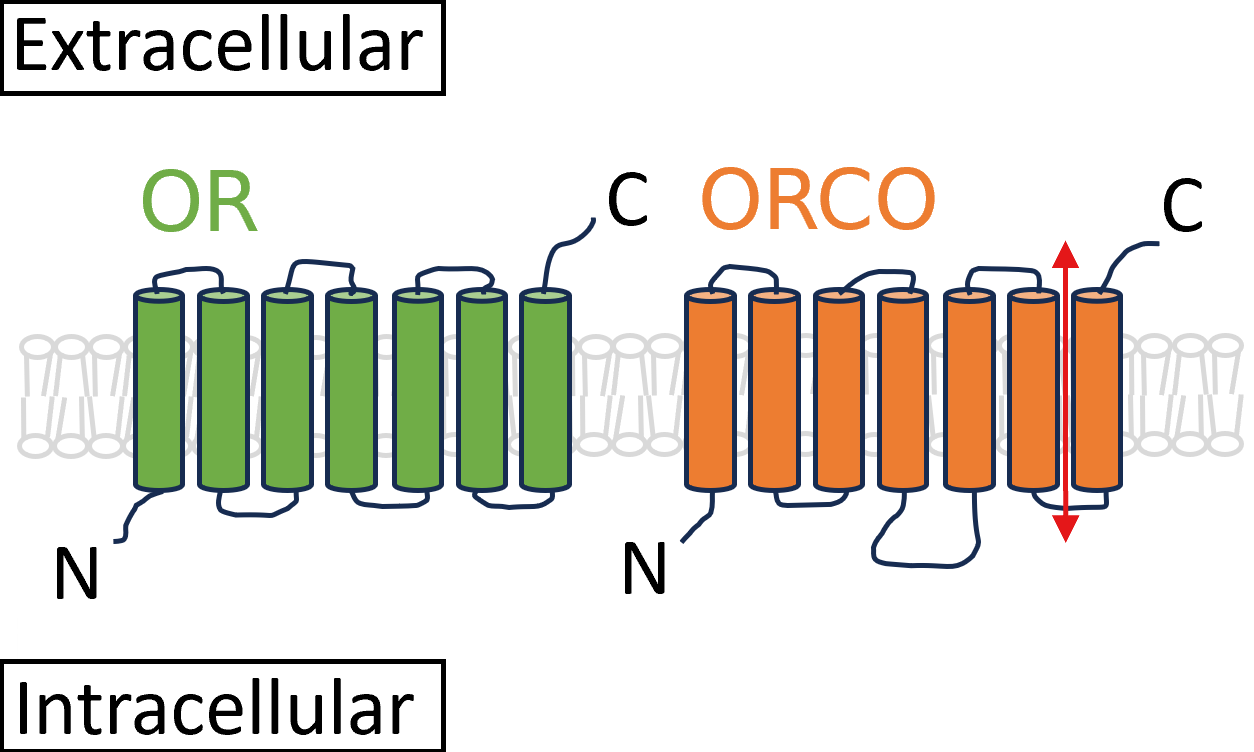
\includegraphics[width=0.65\textwidth,height=\textheight]{figures/ch3/OR_diagram.png}

}

\caption[The tuning OR and odorant receptor coreceptor (ORCO) on the
native cell membrane, with C-terminus and N-terminus
indicated.]{\label{fig-iOR-membrane}The tuning OR and odorant receptor
coreceptor (ORCO) on the native cell membrane, with C-terminus and
N-terminus indicated. The red arrow indicates the location of ion
transport across the membrane.}

\end{figure}

Vertebrate odorant receptor proteins are terminated with an amine group
outside the cell membrane, known as the N-terminus, and terminated with
a carboxyl group inside the cell membrane, known as the C-terminus.
Initially, iORs were thought to be similar in structure to vertebrate
GPCRs \autocite{Clyne1999}, but is now known that iORs have a completely
different topology and mechanism, despite also being a
seven-transmembrane protein. The terminus configuration is inverted: the
C-terminus of the iOR is extracellular, and the N-terminus is
intracellular
\autocite{Smart2008,Glatz2011,Carraher2015,Brito2016,Wicher2021}.
Furthermore, there is no sequence similarity between iORs and GPCRs.
Evolutionarily, insect odorant receptors are thought to be closely
related to insect gustatory receptors (GRs), while they bear no relation
to GPCRs \autocite{Glatz2011,Carraher2015,Wicher2021}. However, despite
iORs not being GPCRs, some interaction between the iOR complex and the
G-protein of the olfactory cell plays a role in odor detection \emph{in
vivo} \autocite{Wicher2008,Wicher2021}. The \emph{in vivo} configuration
of the odorant receptor on the cell membrane, showing the terminus
configuration and location of ORCO ion channel, is illustrated in
Figure~\ref{fig-iOR-membrane}. By testing sensors which incorporate
insect odorant receptors, new information may emerge which helps us to
better understand their atypical structure.

\hypertarget{sensor-functionalisation}{%
\subsection{Sensor Functionalisation}\label{sensor-functionalisation}}

\begin{figure}

\begin{minipage}[t]{0.03\linewidth}

{\centering 

\raisebox{-\height}{


\includegraphics{figures/(a).png}

}

}

\end{minipage}%
%
\begin{minipage}[t]{0.01\linewidth}

{\centering 

~

}

\end{minipage}%
%
\begin{minipage}[t]{0.45\linewidth}

{\centering 

\raisebox{-\height}{

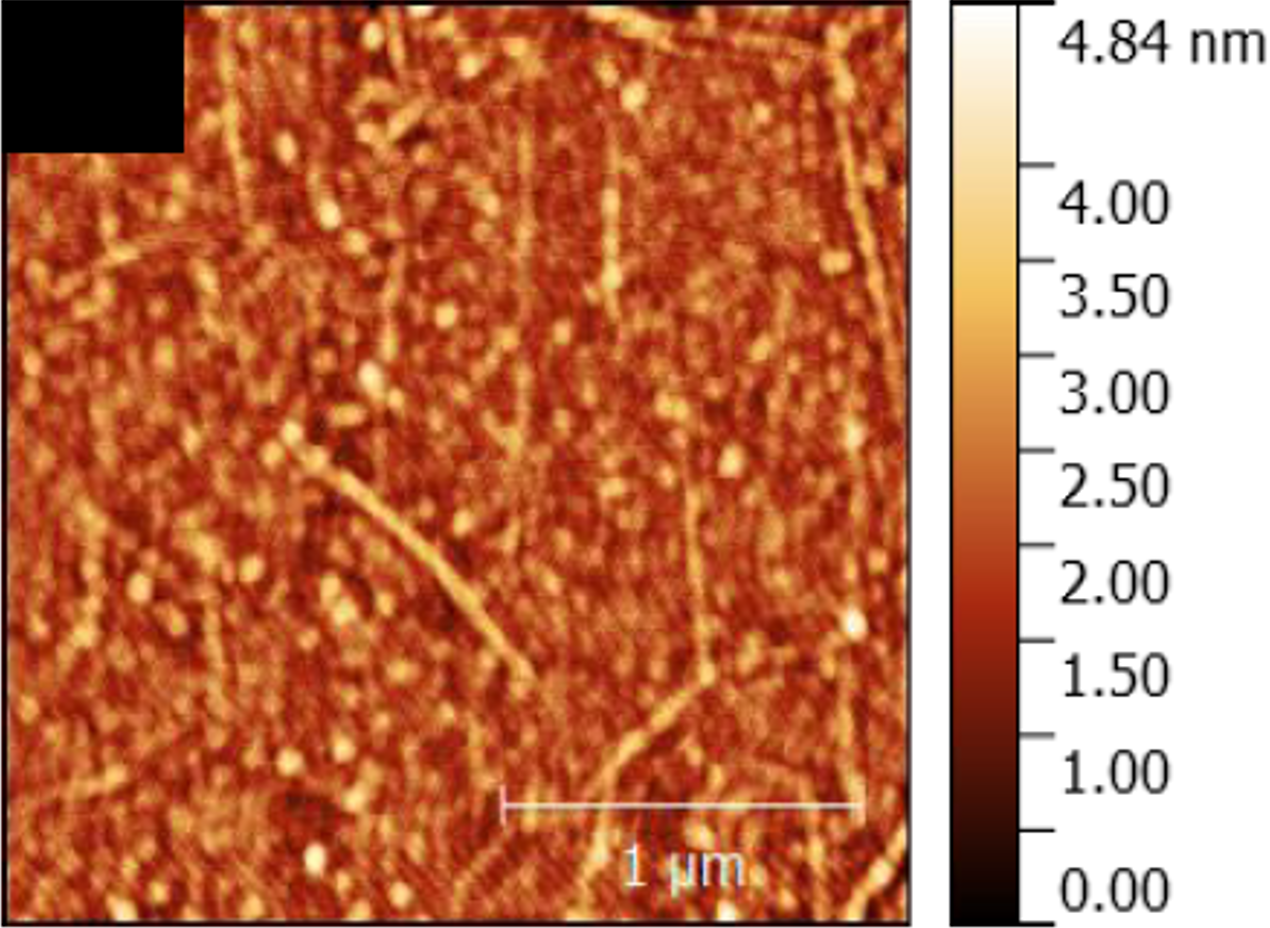
\includegraphics{figures/ch3/pristine_graphene_murugathas.png}

}

}

\end{minipage}%
%
\begin{minipage}[t]{0.01\linewidth}

{\centering 

~

}

\end{minipage}%
%
\begin{minipage}[t]{0.03\linewidth}

{\centering 

\raisebox{-\height}{


\includegraphics{figures/(b).png}

}

}

\end{minipage}%
%
\begin{minipage}[t]{0.01\linewidth}

{\centering 

~

}

\end{minipage}%
%
\begin{minipage}[t]{0.45\linewidth}

{\centering 

\raisebox{-\height}{

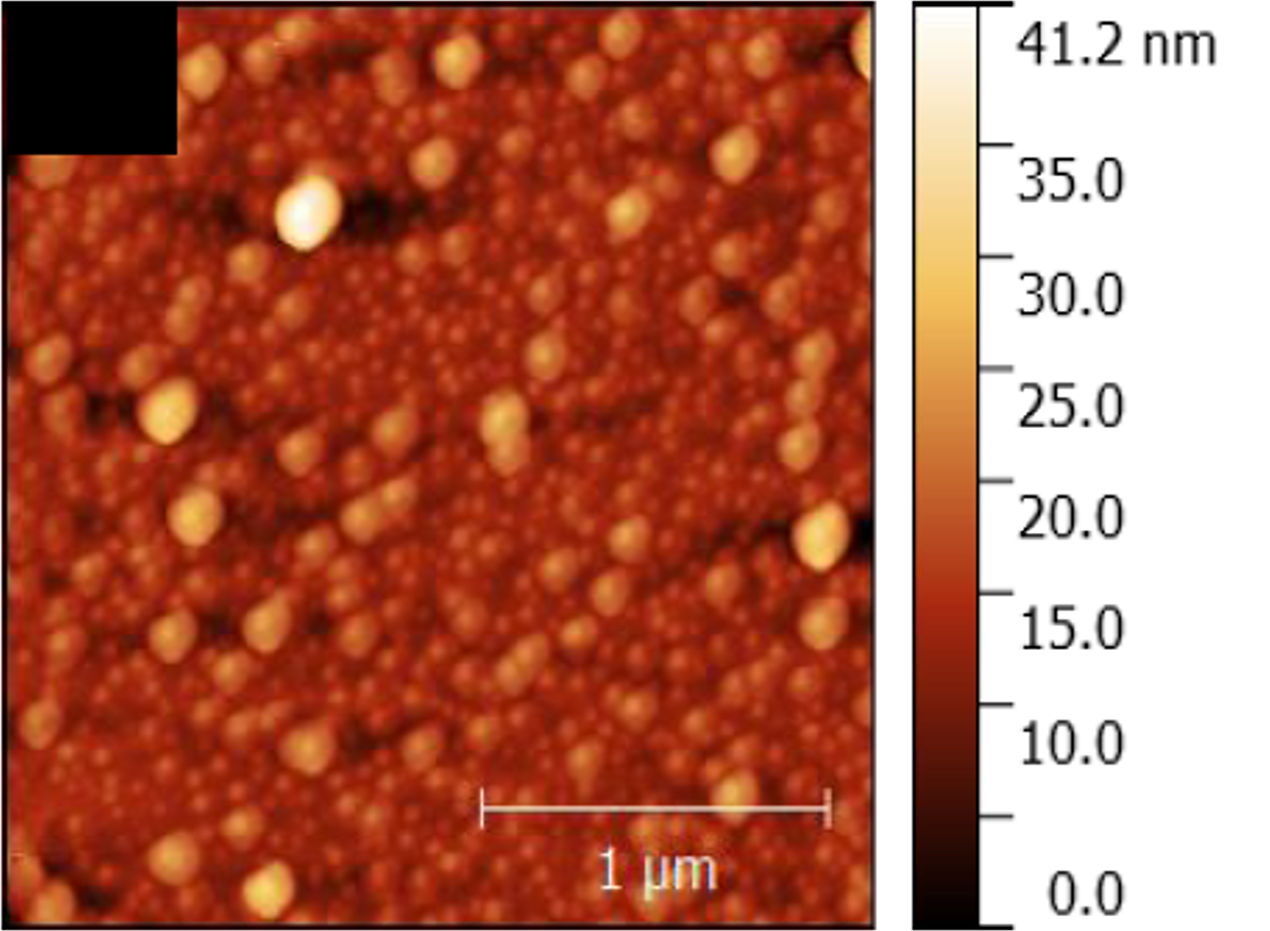
\includegraphics{figures/ch3/OR22a_graphene_murugathas.png}

}

}

\end{minipage}%
%
\begin{minipage}[t]{0.01\linewidth}

{\centering 

~

}

\end{minipage}%
\newline
\begin{minipage}[t]{0.03\linewidth}

{\centering 

\raisebox{-\height}{


\includegraphics{figures/(c).png}

}

}

\end{minipage}%
%
\begin{minipage}[t]{0.01\linewidth}

{\centering 

~

}

\end{minipage}%
%
\begin{minipage}[t]{0.45\linewidth}

{\centering 

\raisebox{-\height}{

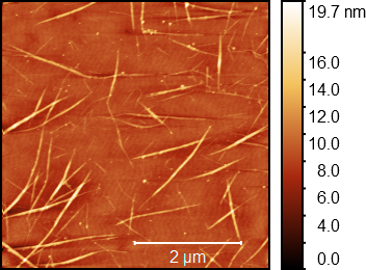
\includegraphics{figures/ch3/pristine_CNT_murugathas.png}

}

}

\end{minipage}%
%
\begin{minipage}[t]{0.01\linewidth}

{\centering 

~

}

\end{minipage}%
%
\begin{minipage}[t]{0.03\linewidth}

{\centering 

\raisebox{-\height}{

\includegraphics{figures/(d).png}

}

}

\end{minipage}%
%
\begin{minipage}[t]{0.01\linewidth}

{\centering 

~

}

\end{minipage}%
%
\begin{minipage}[t]{0.45\linewidth}

{\centering 

\raisebox{-\height}{

\includegraphics{figures/ch3/OR22a_CNT_murugathas.png}

}

}

\end{minipage}%
%
\begin{minipage}[t]{0.01\linewidth}

{\centering 

~

}

\end{minipage}%

\caption[Atomic force microscope images of pristine and
nanodisc-functionalised
thin-films.]{\label{fig-functionalisation-AFM-literature}Atomic force
microscope images of (a) a pristine graphene monolayer, (b) a OR22a
nanodisc-functionalised graphene monolayer, (c) a pristine carbon
nanotube network, and (d) an OR22a nanodisc-functionalised carbon
nanotube network. Reprinted with permission from
\autocite{Murugathas2019a,Murugathas2020}. Copyright \(\copyright\)
2019, 2020 American Chemical Society.}

\end{figure}

Murugathas \emph{et al.} attached a variety of insect odorant receptors
to carbon nanotubes and graphene field-effect transistors using a
nanodisc format. Figure~\ref{fig-functionalisation-AFM-literature} shows
atomic force microscope images of a graphene monolayer before and after
immobilisation of OR22a nanodiscs with PBASE linker in (a) and (b)
respectively, while atomic force microscope images of a randomly
deposited carbon nanotube network before and after OR22a nanodisc
immobilisation with PBASE are shown in (c) and (d) respectively.
Features are seen across the surface of the post-functionalisation image
which are tens of nanometers in height. On the nanotube network, these
features are seen directly next to nanotube bundles, indicating
selective attachment to the nanotubes over the SiO\(_2\) substrate. As
nanodiscs are only 10-20 nm in height, it appears that these features
are large agglomerates of nanodiscs
\autocite{Nath2007,Bayburt2010,Murugathas2019a,Murugathas2020}. As seen
previously for a carbon nanotube network FET in
Section~\ref{sec-odorant-receptors-biosensors}, functionalisation occurs
by non-covalent attachment of PBASE to the channel, and covalent
attachment of the PBASE linker to the odorant receptor amine group. The
nanodisc membrane also possesses amine residues \autocite{Bayburt2010},
so in some cases immobilisation may be directly between the PBASE linker
and nanodisc membrane.

\begin{figure}

\begin{minipage}[t]{0.03\linewidth}

{\centering 

\raisebox{-\height}{

\includegraphics{figures/(a).png}

}

}

\end{minipage}%
%
\begin{minipage}[t]{0.01\linewidth}

{\centering 

~

}

\end{minipage}%
%
\begin{minipage}[t]{0.45\linewidth}

{\centering 

\raisebox{-\height}{

\includegraphics{figures/ch3/OR22a_ND_GFET.png}

}

}

\end{minipage}%
%
\begin{minipage}[t]{0.01\linewidth}

{\centering 

~

}

\end{minipage}%
%
\begin{minipage}[t]{0.03\linewidth}

{\centering 

\raisebox{-\height}{

\includegraphics{figures/(b).png}

}

}

\end{minipage}%
%
\begin{minipage}[t]{0.01\linewidth}

{\centering 

~

}

\end{minipage}%
%
\begin{minipage}[t]{0.45\linewidth}

{\centering 

\raisebox{-\height}{

\includegraphics{figures/ch3/OR22a_ND_CNTFET.png}

}

}

\end{minipage}%
%
\begin{minipage}[t]{0.01\linewidth}

{\centering 

~

}

\end{minipage}%
\newline
\begin{minipage}[t]{0.03\linewidth}

{\centering 

\raisebox{-\height}{

\includegraphics{figures/(c).png}

}

}

\end{minipage}%
%
\begin{minipage}[t]{0.01\linewidth}

{\centering 

~

}

\end{minipage}%
%
\begin{minipage}[t]{0.45\linewidth}

{\centering 

\raisebox{-\height}{

\includegraphics{figures/ch3/Empty_ND_GFET.png}

}

}

\end{minipage}%
%
\begin{minipage}[t]{0.01\linewidth}

{\centering 

~

}

\end{minipage}%
%
\begin{minipage}[t]{0.03\linewidth}

{\centering 

\raisebox{-\height}{

\includegraphics{figures/(d).png}

}

}

\end{minipage}%
%
\begin{minipage}[t]{0.01\linewidth}

{\centering 

~

}

\end{minipage}%
%
\begin{minipage}[t]{0.45\linewidth}

{\centering 

\raisebox{-\height}{

\includegraphics{figures/ch3/Empty_ND_CNTFET.png}

}

}

\end{minipage}%
%
\begin{minipage}[t]{0.01\linewidth}

{\centering 

~

}

\end{minipage}%

\caption[Transfer characteristic curves of graphene and carbon nanotube
network field-effect transistors before and after either OR22a or empty
nanodisc
functionalisation.]{\label{fig-functionalisation-literature}Transfer
characteristic curves before and after functionalisation of (a) an OR22a
nanodisc-functionalised graphene field-effect transistor, (b) an OR22a
nanodisc-functionalised CNT network FET, (c) an empty
nanodisc-functionalised graphene FET and (d) an empty
nanodisc-functionalised CNT network FET. Reproduced with permission from
\autocite{Murugathas2019a,Murugathas2020}.}

\end{figure}

Functionalisation of a FET device channel with iORs significantly alters
the transfer characteristics of that channel. Murugathas \emph{et al.}
found that successful functionalisation of a CNT FET device with iORs
would typically increase the device on-current, increase its on-off
ratio and cause a significant negative shift in threshold voltage, as
shown in Figure~\ref{fig-functionalisation-literature} (a)
\autocite{Murugathas2019a}. Meanwhile, successful functionalisation of a
graphene device with iORs would typically dramatically decrease the
device on-current and cause a negative shift in Dirac voltage, as seen
in Figure~\ref{fig-functionalisation-literature} (b)
\autocite{Murugathas2020}. These changes are not simply the result of
linker attachment to the channel surface \autocite{Murugathas2019a}. It
is thought that the negative shift of both threshold and Dirac voltages
are caused by the N-terminus amine groups on the odorant receptors or
amine groups on the nanodisc membrane scaffold proteins donating
electrons to the device channel, which has a similar effect to doping
the channel with impurities
\autocite{Bradley2004,Murugathas2019a,Murugathas2020}. Note that very
similar changes occur when functionalising with empty nanodiscs which
contain no odorant receptors, shown in
Figure~\ref{fig-functionalisation-literature} (c) and
Figure~\ref{fig-functionalisation-literature} (d). Unless the odorant
receptors attach preferentially to the network over nanodiscs, it
appears the gating effect is predominantly due to the large-scale
attachment of nanodisc membranes.

\hypertarget{sensing-behaviour}{%
\subsection{Sensing Behaviour}\label{sensing-behaviour}}

\begin{figure}

\begin{minipage}[t]{0.03\linewidth}

{\centering 

\raisebox{-\height}{

\includegraphics{figures/(a).png}

}

}

\end{minipage}%
%
\begin{minipage}[t]{0.01\linewidth}

{\centering 

~

}

\end{minipage}%
%
\begin{minipage}[t]{0.45\linewidth}

{\centering 

\raisebox{-\height}{

\includegraphics{figures/ch3/OR22a_realtime_normalised_GFET_1.png}

}

}

\end{minipage}%
%
\begin{minipage}[t]{0.01\linewidth}

{\centering 

~

}

\end{minipage}%
%
\begin{minipage}[t]{0.03\linewidth}

{\centering 

\raisebox{-\height}{

\includegraphics{figures/(b).png}

}

}

\end{minipage}%
%
\begin{minipage}[t]{0.01\linewidth}

{\centering 

~

}

\end{minipage}%
%
\begin{minipage}[t]{0.45\linewidth}

{\centering 

\raisebox{-\height}{

\includegraphics{figures/ch3/OR22a_realtime_normalised_CNTFET_1.png}

}

}

\end{minipage}%
%
\begin{minipage}[t]{0.01\linewidth}

{\centering 

~

}

\end{minipage}%
\newline
\begin{minipage}[t]{0.03\linewidth}

{\centering 

\raisebox{-\height}{

\includegraphics{figures/(c).png}

}

}

\end{minipage}%
%
\begin{minipage}[t]{0.01\linewidth}

{\centering 

~

}

\end{minipage}%
%
\begin{minipage}[t]{0.45\linewidth}

{\centering 

\raisebox{-\height}{

\includegraphics{figures/ch3/OR22a_realtime_normalised_GFET_2.png}

}

}

\end{minipage}%
%
\begin{minipage}[t]{0.01\linewidth}

{\centering 

~

}

\end{minipage}%
%
\begin{minipage}[t]{0.03\linewidth}

{\centering 

\raisebox{-\height}{

\includegraphics{figures/(d).png}

}

}

\end{minipage}%
%
\begin{minipage}[t]{0.01\linewidth}

{\centering 

~

}

\end{minipage}%
%
\begin{minipage}[t]{0.45\linewidth}

{\centering 

\raisebox{-\height}{

\includegraphics{figures/ch3/OR22a_realtime_normalised_CNTFET_2.png}

}

}

\end{minipage}%
%
\begin{minipage}[t]{0.01\linewidth}

{\centering 

~

}

\end{minipage}%

\caption[Real-time sensing behaviour of graphene and carbon nanotube
network field-effect transistors before and after OR22a
functionalisation.]{\label{fig-iOR-sensing-literature}Real-time
responses to concentrations of methyl hexanoate in \(1 \times\)
phosphate buffer saline (PBS) with 1\% v/v DMSO by (a) an OR22a
nanodisc-functionalised graphene field-effect transistor and (b) an
OR22a nanodisc-functionalised CNT network FET, alongside the normalised
signal response curves corresponding to (c) graphene FETs and (d) carbon
nanotube network FETs. The response curves show the cumulative responses
of OR22a-functionalised devices to both the positive ligand methyl
hexanoate (green) and negative ligand \emph{trans}-2-hexan-1-al (black).
They also show the cumulative response of a empty nanodisc
functionalised device to methyl hexanoate (purple). Reproduced with
permission from \autocite{Murugathas2019a,Murugathas2020}.}

\end{figure}

Figure~\ref{fig-iOR-sensing-literature} (a) and (b) show the respective
responses of the OR22a-functionalised graphene FET and CNT FET to
various concentrations of methyl hexanoate in real-time. This result
demonstrates that iOR-FETs are sensitive down to the femtomolar scale in
an aqueous environment. Figure~\ref{fig-iOR-sensing-literature} (c) and
(d) compare the dose dependent responses to methyl hexanoate from
multiple OR22a-functionalised devices to that of relevant controls. It
was verified that the OR22a-functionalised devices would not respond to
\emph{trans}-2-hexan-1-al, the negative ligand for OR22a; it was also
verified that empty nanodiscs would not respond non-selectively to the
positive ligand \autocite{Murugathas2019a,Murugathas2020}. It is notable
that unlike iORs \emph{in vivo}, ORCO does not appear to be required for
the bioelectronic nose to function
\autocite{Murugathas2019a,Murugathas2020,Khadka2019,Cheema2021}.
Furthermore, G-protein signaling pathways are not required
\autocite{Sato2014}. It has been proposed that the signal response
results from the positive ligand binding to the iOR protein, causing a
change in conformation, the same mechanism underpinning the behaviour of
many of the vertebrate odorant receptor sensors seen in
Section~\ref{sec-odorant-receptors-biosensors}. Cheema \emph{et al.}
used neutron reflectometry to demonstrate that OR22a nanodiscs undergo a
1 nm height change after ethyl hexanoate exposure, likely resulting from
a structural change \autocite{Cheema2021}.

This change most likely affects the channel in one of two ways. The
first involves transfer of charge from the iOR to the channel, reducing
I\(_{d}\) and causing a negative threshold voltage (or Dirac point)
shift. Another could be a more indirect electrostatic gating effect from
movement of charge within the Debye screening length of the channel. The
Debye length of \(1 \times\) PBS buffer is typically much shorter than
the height of a single nanodisc \autocite{Murugathas2019a}. However, if
structural changes in the iOR were primarily occurring at its base, it
is still possible that the electrostatic gating could be the primary
sensing mechanism. From further development and examination of iOR-based
biosensors, new insights into the mechanisms underlying the nanodisc
signal transduction may emerge \autocite{Glatz2011}. As discussed here,
the literature has primarily focused on the operation of iOR carbon
nanotube and graphene FET biosensors in an aqueous environment
\autocite{Murugathas2019a,Murugathas2020}. It is as yet unknown whether
insect odorant receptors can operate in a vapour-phase environment, but
this possibility is explored in this thesis.

\hypertarget{sec-non-specific-binding}{%
\section{Non-Specific Binding}\label{sec-non-specific-binding}}

Non-specific binding (NSB) refers to any attachment within the sensing
environment not related to the specific analyte of interest
\autocite{Lichtenberg2019,Shkodra2021}. Non-specific binding is
particularly significant for protein-functionalised devices. Proteins
may be spontaneously adsorbed onto carbon nanotube or graphene surfaces
during functionalisation in a manner which is not linker-mediated
\autocite{Bradley2004,Star2003a,Chen2004}. Non-covalently bound proteins
may detach and reattach to available surfaces in a non-specific manner
when exposed to a high ionic strength electrolyte post-functionalisation
\autocite{Dung2018}. Non-specific binding may also result from
protein-protein interactions, misoriented attachment of proteins,
attachment to a sticky substrate \autocite{Chen2004,Lichtenberg2019}. It
can also result from electrostatic binding to any charged surface
present, such as the gold electrodes \autocite{Garcia-Aljaro2010} or
Ag/AgCl reference electrode
\autocite{Chen2004,Minot2007,Lichtenberg2019}. Liquid-gated graphene and
carbon nanotube devices are highly sensitive to the approach of charge
within the Debye length of the device channel, and so non-specific
adsorption can lead to spurious signals during sensing
\autocite{Star2003a,Chen2004,Lichtenberg2019,Shkodra2021}. A variety of
measures can be taken to prevent NSB from occurring. Once bioreceptors
have been attached to the channel, remaining exposed carbon nanotubes
can be passivated with chemical coatings such as Tween-20
\autocite{Chen2004}, PEG
\autocite{Star2003a,Lee2012b,Gao2016,Filipiak2018}, and ethanolamine
\autocite{Maehashi2007,Das2011}.

\hypertarget{summary}{%
\section{Summary}\label{summary}}

Odorant receptors can be used to fabricate highly sensitive and
selective biosensors using carbon nanotube and graphene field-effect
transistors as the transducer element. Both vertebrate and insect
odorant receptors are seven-transmembrane proteins, but each has a
different sequence and have inverted terminus positions relative to the
cell membrane wall \emph{in vivo}. Insect odorant receptor detection
\emph{in vivo} differs significantly from vertebrate OR detection, with
an ORCO-mediated ion channel involved. ORs can be held in the native
cell membrane for sensor applications, but artificial lipid bilayer
formats such as micelles, nanovesicles or nanodiscs are generally
preferred due to their enhanced stability. Mammalian odorant receptors
have been thoroughly explored in carbon nanotube and graphene
field-effect transistor sensing applications, with both non-covalent and
covalent functionalisation mechanisms used to create sensors which
detect analyte at sub-femtomolar concentrations. The mechanisms behind
sensing rely on transistor gating either due to ion flow into a
nanovesicle format, or a conformational change in the odorant receptor.
Covalently-attached mammalian odorant receptors have also been used for
vapour-phase detection with a single carbon nanotube field-effect
transistor device at concentrations down to \(\sim\) 7 ppb by Goldsmith
\emph{et al.}

Femtomolar detection of analyte has also been achieved with an insect
odorant receptor functionalised device. However, the exact mechanism
behind detection is unclear, as the presence of ORCO is not required for
successful sensor behaviour. It is possible that the mechanism results
from a change in conformation of the odorant receptor, similar to the
mammalian odorant receptor. Due to the possible difference in mechanism
between mammalian odorant receptor detection and insect odorant receptor
detection, it is not clear that vapour-phase detection can be achieved
by simply reproducing the work of Goldsmith \emph{et al.} using insect
odorant receptors. \textbf{?@sec-noncovalent-functionalisation} looks
further at various non-covalent functionalisation approaches for the
creation of a insect odorant receptor-based field-effect transistor
biosensor, while \textbf{?@sec-biosensing-iORs} tests sensor behaviour
in both aqueous and vapour-phase environments.

\cleardoublepage
\phantomsection
\addcontentsline{toc}{part}{Appendices}
\appendix

\hypertarget{references}{%
\chapter*{References}\label{references}}
\addcontentsline{toc}{chapter}{References}

\markboth{References}{References}

\begingroup
\raggedright

\printbibliography[heading=none]

\endgroup

\newpage{}

\hfill\break

\thispagestyle{empty}

\mbox{~} \clearpage \newpage


\backmatter

\end{document}
